\documentclass{article} 
\usepackage[utf8]{inputenc}
\usepackage[margin=2.5cm]{geometry} % decrease the margin size

\usepackage{hyperref} % to include weblinks

\usepackage{graphicx} % handle images and figures
\usepackage{placeins} % to control placement of figures

\usepackage{amsmath} % general package for writing math
\usepackage{amsfonts} % math fonts for obscure symbols
\usepackage{mathabx}
\usepackage[version=4]{mhchem}

\usepackage[nottoc]{tocbibind}
\usepackage[backend=biber,dateabbrev=false]{biblatex} % package for handling references
\addbibresource{references.bib}
\usepackage{csquotes}

\usepackage{fancyhdr}

\setlength{\parindent}{0pt} % remove indentation at the beginning of pargraphs

\begin{document}

\pagestyle{fancy}
\setlength{\headheight}{15pt}
\fancyhead[L]{Dynamic Light Scattering}
\fancyhead[R]{Louis-Hendrik Barboutie, Rajon Bhuyan}

\begin{titlepage}
    \begin{center}
        \vspace*{1cm}
        \Huge
        \textbf{Dynamic Light Scattering}
        
        \vspace{0.5cm}
        \LARGE
        Physikalisches Praktikum für Fortgeschrittene I
        
        \vspace{1.5cm}
        \textbf{Louis-Hendrik Barboutie and Rajon Bhuyan} \newline
        \textbf{7016306 \& 7029677}
        
        \vspace{0.5cm}
        \Large 
        Supervisor: Timothée Boutfol
        
        \vfill

        
\includegraphics[width=0.4\textwidth]{logo_uni.png}
        
        \Large
        11$^{\underline{\text{th}}}$ November 2022
    \end{center}
\end{titlepage}

\tableofcontents
\newpage

\section{Introduction}
Dynamic Light Scattering (DLS) is an effective method for measuring the size of particles in solutions, based on their brownian motion. Other applications include the determination of viscosities of solvents using known particle sizes, or studying the surface structure of particles, by eg. determining whether adsorbed polymers are aligned parallel or orthogonal to the membrane of a particle. It does however not work with any particle size: as later discussed, one can differentiate several regimes where DLS is possible. 

The particle size one can calculate with DLS is not the actual size of the particle. Macromolecules and other particles can have all kinds of shapes, but in DLS one assumes each particle to be spherical. Therefore the size one obtains is the one of a spherical particle whose movement corresponds to that of the observed particle.

Most of the time one is looking at solutions containing particles of one size, but it is also possible to do DLS with solutions containing multiple particle sizes. If the size difference is too large, one may encounter the risk that the scattered light from the bigger particles overshadows the scattered light from the smaller particles. It is then difficult to analyze the data as the contribution of the smaller particles is extremely small in comparison to the contribution from the bigger particles.

Since the viscosity of a fluid is dependent on the temperature, DLS is very sensible to thermal fluctuations and controlling this parameter is very important. Another factor which may impact the experiment is the ionic concentration in the solution, as ions may interact with the particles. A possibility to counteract this is to add salt (\ce{NaCl}) to the solutions. 

The motion of the particles is not directly studied in DLS, but rather the temporal correlation of the scattered light. This is in contrast to static light scattering, where one looks at the average of the scattered light's intensity, which does not allow the determination of particle size. 

\section{Theory}

\subsection{Light scattering}
Light is an electromagnetic wave, and what we actually measure during experiments is not its amplitude  $\Vec{E}_S$ but its intensity $I_S = |\Vec{E}_S|^2$.

When scattering light with wavelength $\lambda$ through a sample which contains particles of diameter $d$, we can differentiate two regimes:
\begin{enumerate}
    \item Rayleigh regime: $d < \frac{\lambda}{10}$ [nm] \newline
    The scattered light is isotropic, which means the light is emitted equally in all directions and thus independent of measuring angle.
    
    \item Mie regime: $d > \frac{\lambda}{10}$ [nm] \newline
    The scattering of light is anisotropic, there are preferred scattering directions, which indicate an angular dependency.
\end{enumerate}

There is also the case in which $d \approx \lambda$, but it is very complicated and isn't in the scope of this experiment.

Light scattering is sensible to various properties of the solution. Most notably, to the refractive index of the solvent and to the concentration of the particles. It is in fact tiny variations in concentrations of particles which lead to scattering. One can derive the so-called absolute scattering intensity:
\begin{equation}
    R = \frac{4\pi^2}{\lambda^4}n_{D,0}^2 \left( \frac{\partial n_D^2}{\partial c} \right) \frac{cM}{N_L}
\end{equation}
Where:
\begin{itemize}
    \item $\lambda$ = wavelength of the scattered light
    \item $n_{D,0}$ = refractive index of the solvent
    \item $n_D$ = refractive index of solute
    \item $c$ = concentration of the solute
\end{itemize}
This quantity is independent of most other physical variables, most notably of the scattering angle. \\

Depending on the particle size, the scattering foci inside of the particle may overlap, leading to constructive interference when scattering light. When the light is in phase opposition, destructive scattering occurs.
Particles of diameter $d > \frac{\lambda}{10}$ nm do not scatter light isotropically, and one can define the scattering vector:
\begin{align}
    \Vec{q} &= \Vec{k} - \Vec{k}_0\\
    |\Vec{q}| &= \frac{4 \pi n_D}{\lambda} \sin\left(\frac{\theta}{2}\right)
\end{align}
Because destructive interference is occurring, the resulting intensity is dependent on the angle of measurement.

\subsection{Brownian motion}
Particles follow so-called Brownian motion when in a liquid. They follow an erratic path which makes them move in random directions. To a particle we can associate a diffusion coefficient, given by the Stokes-Einstein equation:

\begin{equation}
    D_S = \frac{k_B T}{6 \pi \eta r_H}
\end{equation}

Where: \begin{itemize}
    \item $k_B =$ Boltzmann constant
    \item $T =$ temperature of the solution
    \item $\eta =$ viscosity of the solvent
    \item $r_H =$ hydrodynamic radius of the particle 
\end{itemize}

Due to the random nature of their movement, the particles do not move away from their initial position on average, therefore the mean displacement $\langle \Delta R(\tau) \rangle = cst$. So we look at the mean displacement square, so that we lose information about the direction of the walk, but gain more information about the total distance travelled. It is also linked to the diffusion coefficient by the following relationship:
\begin{equation}
    \langle (\Delta R(\tau))^2 \rangle = 6 D_S \tau
\end{equation}

\subsection{Dynamic Light Scattering (DLS)}
The Brownian motion leads to interparticular interference of the scattered light between different particles. The randomness of their motion can be seen in the scattering amplitude $I(q,t)$. One can then correlate the amplitudes, ie. make a comparison how much the intensity at a time $t$ overlaps with the intensity at time $t+\tau$ with the correlation function $f(q,\tau) = \langle I(q,t)I(q,t+\tau)\rangle$. The normalized amplitude correlation function is then given by:
\begin{equation}
    F_S(q,\tau) = \sqrt{\frac{\langle I(q,t)I(q,t+\tau) \rangle}{\langle I(q,t) \rangle ^2}-1}
\end{equation}
Furthermore, the correlation function can also be linked to the diffusion coefficient by:
\begin{equation}
    F_S(q,\tau) = e^{-D_S q^2 \tau}
\end{equation}

\subsection{Mono- and poly-disperse samples}
Solutions may have different sized beads inside of them. We can associate a single diffusion coefficient to mono-disperse solutions. In poly-disperse solutions however, there are several dispersion coefficients associated to each particle size. The resulting correlation function is an overlap of several individual correlation function for each particle size. We can nonetheless identify an apparent diffusion coefficient, which is obtained by considering a poly-disperse solution and treating it as a mono-disperse solution, for small intervals of time. 

\subsection{Solving for the hydrodynamic radius}

For a solution containing particles of a single size, we can fit the autocorrelation function with a function of the form:
\begin{equation}
    f(t) = A + Be^{-2 \Gamma t}
    \label{eq:SingleParticleFit}
\end{equation}

Or alternatively for a solution containing two populations of different sizes:
\begin{equation}
    f(t) = A + Be^{-2 \Gamma_1 t} + Ce^{-2 \Gamma_2 t}
    \label{eq:DoubleParticleFit}
\end{equation}

Where $\Gamma_i = q^2 D_i$. One can then solve for the hydrodynamic radius using the norm of $\Vec{q}$: \begin{equation}
    q = \frac{4 \pi n_0}{\lambda_0}\sin{\frac{\theta}{2}}
\end{equation}
\begin{equation}
    r_H = \frac{4 \pi k_B T}{3 \eta \Gamma} \left( \frac{n_0}{\lambda_0} \sin \left( \frac{\theta}{2} \right) \right)^2
\end{equation}

The values of the constants in the above equation are the following:

\begin{itemize}
    \item $\lambda_0 = 633$ nm
    \item $\eta = 1,0016 \cdot 10^{-3} \ \text{Pa} \cdot \text{s}$ \cite{ViscosityH2O}
    \item $k_B = 1,380649 \cdot 10^{-23} \ \text{J} \cdot \text{K}^{-1}$
    \item $T = 298 \ \text{K}$
    \item $n_0 = 1.333$ \cite{RefractiveIndexH2O}
\end{itemize}

\newpage
\section{Setup}
The setup for the experiment can be seen in fig. \ref{fig:Setup}. Both the laser on the left and the sample holder in the center of the construction are fixed. The arm on the right holds the detector, and its rotation with respect to the laser can be adjusted from 0° to 90°. The signal from the detector is then fed to the correlator and finally relayed to the computer for data acquisition and analysis. Each sample needs to be transferred into a small cuvette, which is slid into the central holder. The laser beam hits the solution directly, but its intensity is reduced via two filters, so as not to damage the detector. The light from the laser is supposed to be focused through a biconvex lens, which was however missing during our experiment. When doing the measurements, a cardboard box can be put over the setup, to avoid eye damage from the laser.

\begin{figure}[!ht]
    \centering
    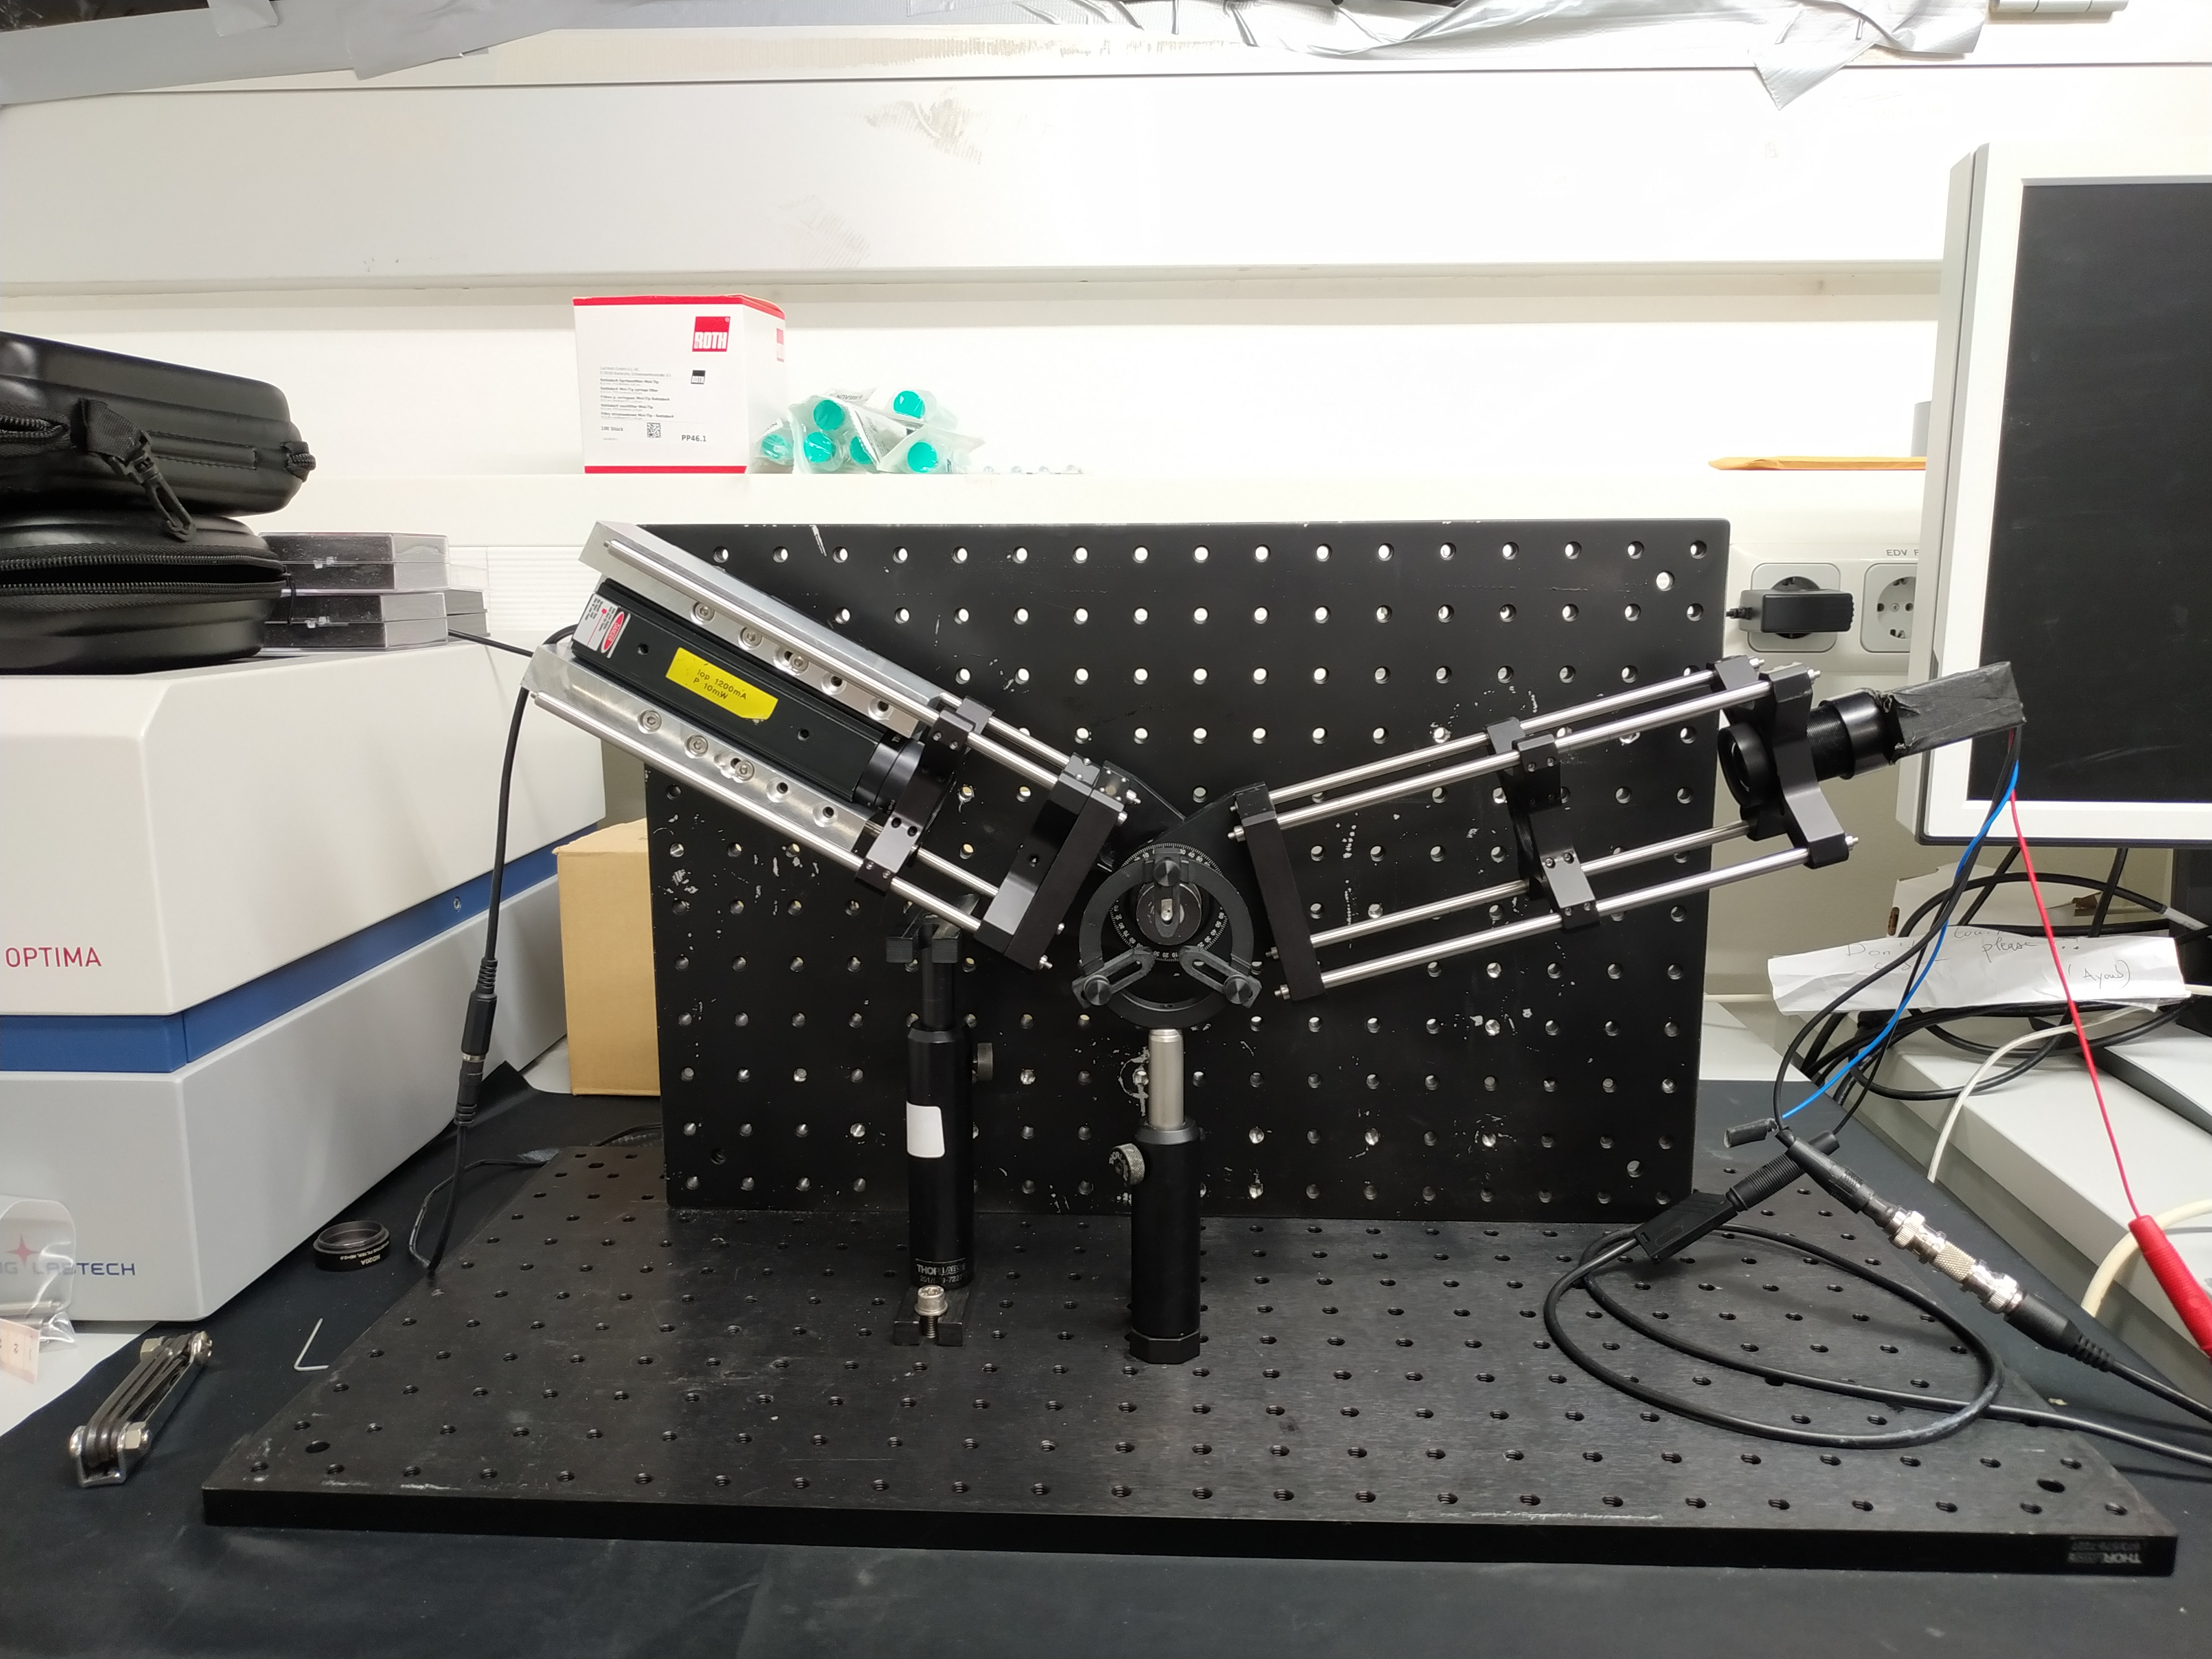
\includegraphics[width=0.7\textwidth]{1_DynamicLightScattering/Graphics/Setup_DLS.jpg}
    \caption{Setup for the DLS Experiment}
    \label{fig:Setup}
\end{figure}
\FloatBarrier

\section{Sample preparation}

A total of six samples are prepared according to the lab guide:
\begin{itemize}
    \item Sample 1: Latex I, $\diameter$ 100 nm
    \item Sample 2: Latex II, $\diameter$ 460 nm
    \item Sample 3: Ludox, $\diameter$ 10 nm
    \item Sample 5: Latex I, $\diameter$ 100 nm, diluted sample 1
    \item Sample 6: Latex I, $\diameter$ 100 nm, diluted sample 5
    \item Sample 7: Latex I, $\diameter$ 100 nm, Latex II, $\diameter$ 460 nm
\end{itemize}

Since we don't know the concentrations of the initial solutions, it is impossible to give quantitative values on the concentration of the diluted samples.

\newpage
\section{Results}

\subsection{Particle sizes}

We record the correlation function of the samples 1, 2 and 3 at scattering angles of 45°, 60°, 75° and 90°. Each correlation function is then fitted using the equation for a single particle size (eq. \ref{eq:SingleParticleFit}).

\subsubsection{Sample 1}
The correlation functions and fits obtained for sample 1 are plotted in fig. \ref{fig:CorrFctProbe1} and the calculated diameters are presented in fig. \ref{fig:RadiiProbe1} and tab. \ref{tab:DiametersSample1}. 
The correlation data for 60° and 90° overlap, which is most likely due to the fact we saved the wrong data file. After calculating the diameter of the particles, one can clearly see in fig. \ref{fig:RadiiProbe1}, that the value obtained for an angle of 90° is an outlier.

The calculated diameter also has an angular dependency: as the angle increases, the diameter decreases (dismissing the data point for 90°). 

Sample 1 contains a solution of particles with a diameter of 100 nm, however our measurements indicate a diameter of the order of magnitude of 50 nm.

\begin{figure}[!ht]
    \centering
    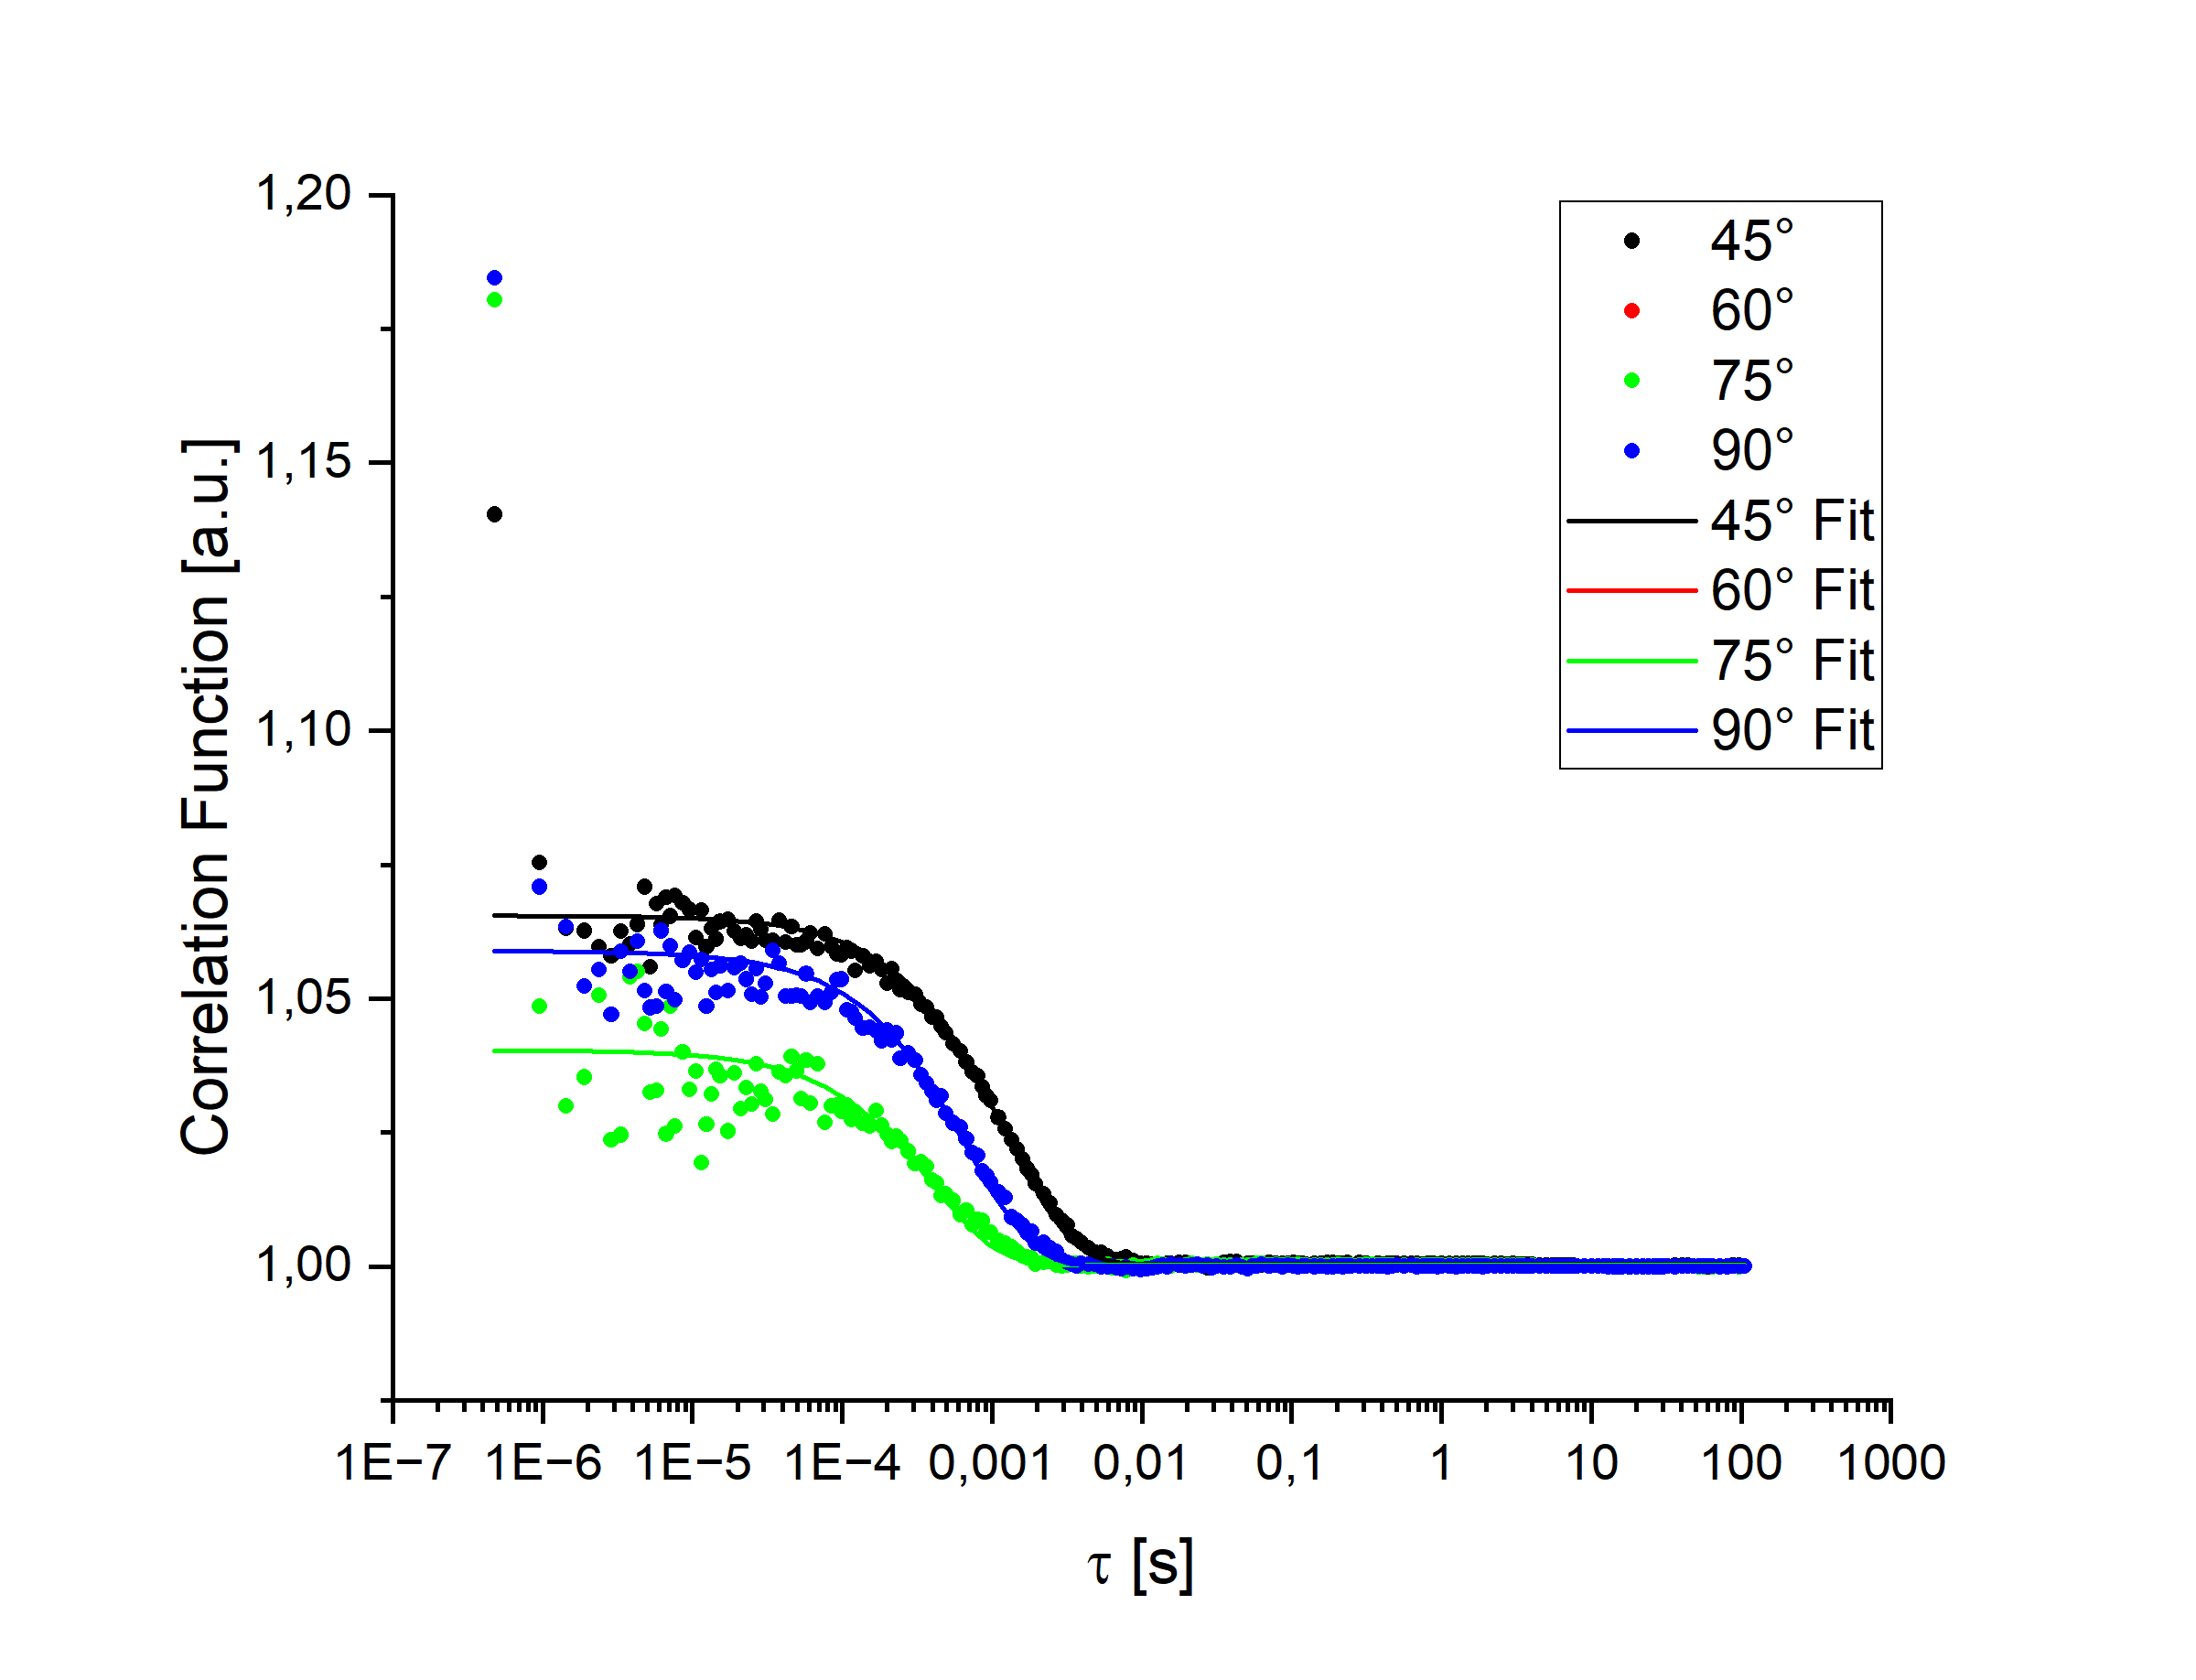
\includegraphics[width=0.8\textwidth]{1_DynamicLightScattering/Graphics/CorrFctProbe1.png}
    \caption{Correlation functions for sample 1 at different scattering angles}
    \label{fig:CorrFctProbe1}
\end{figure}
\FloatBarrier

\begin{figure}[!ht]
    \centering
    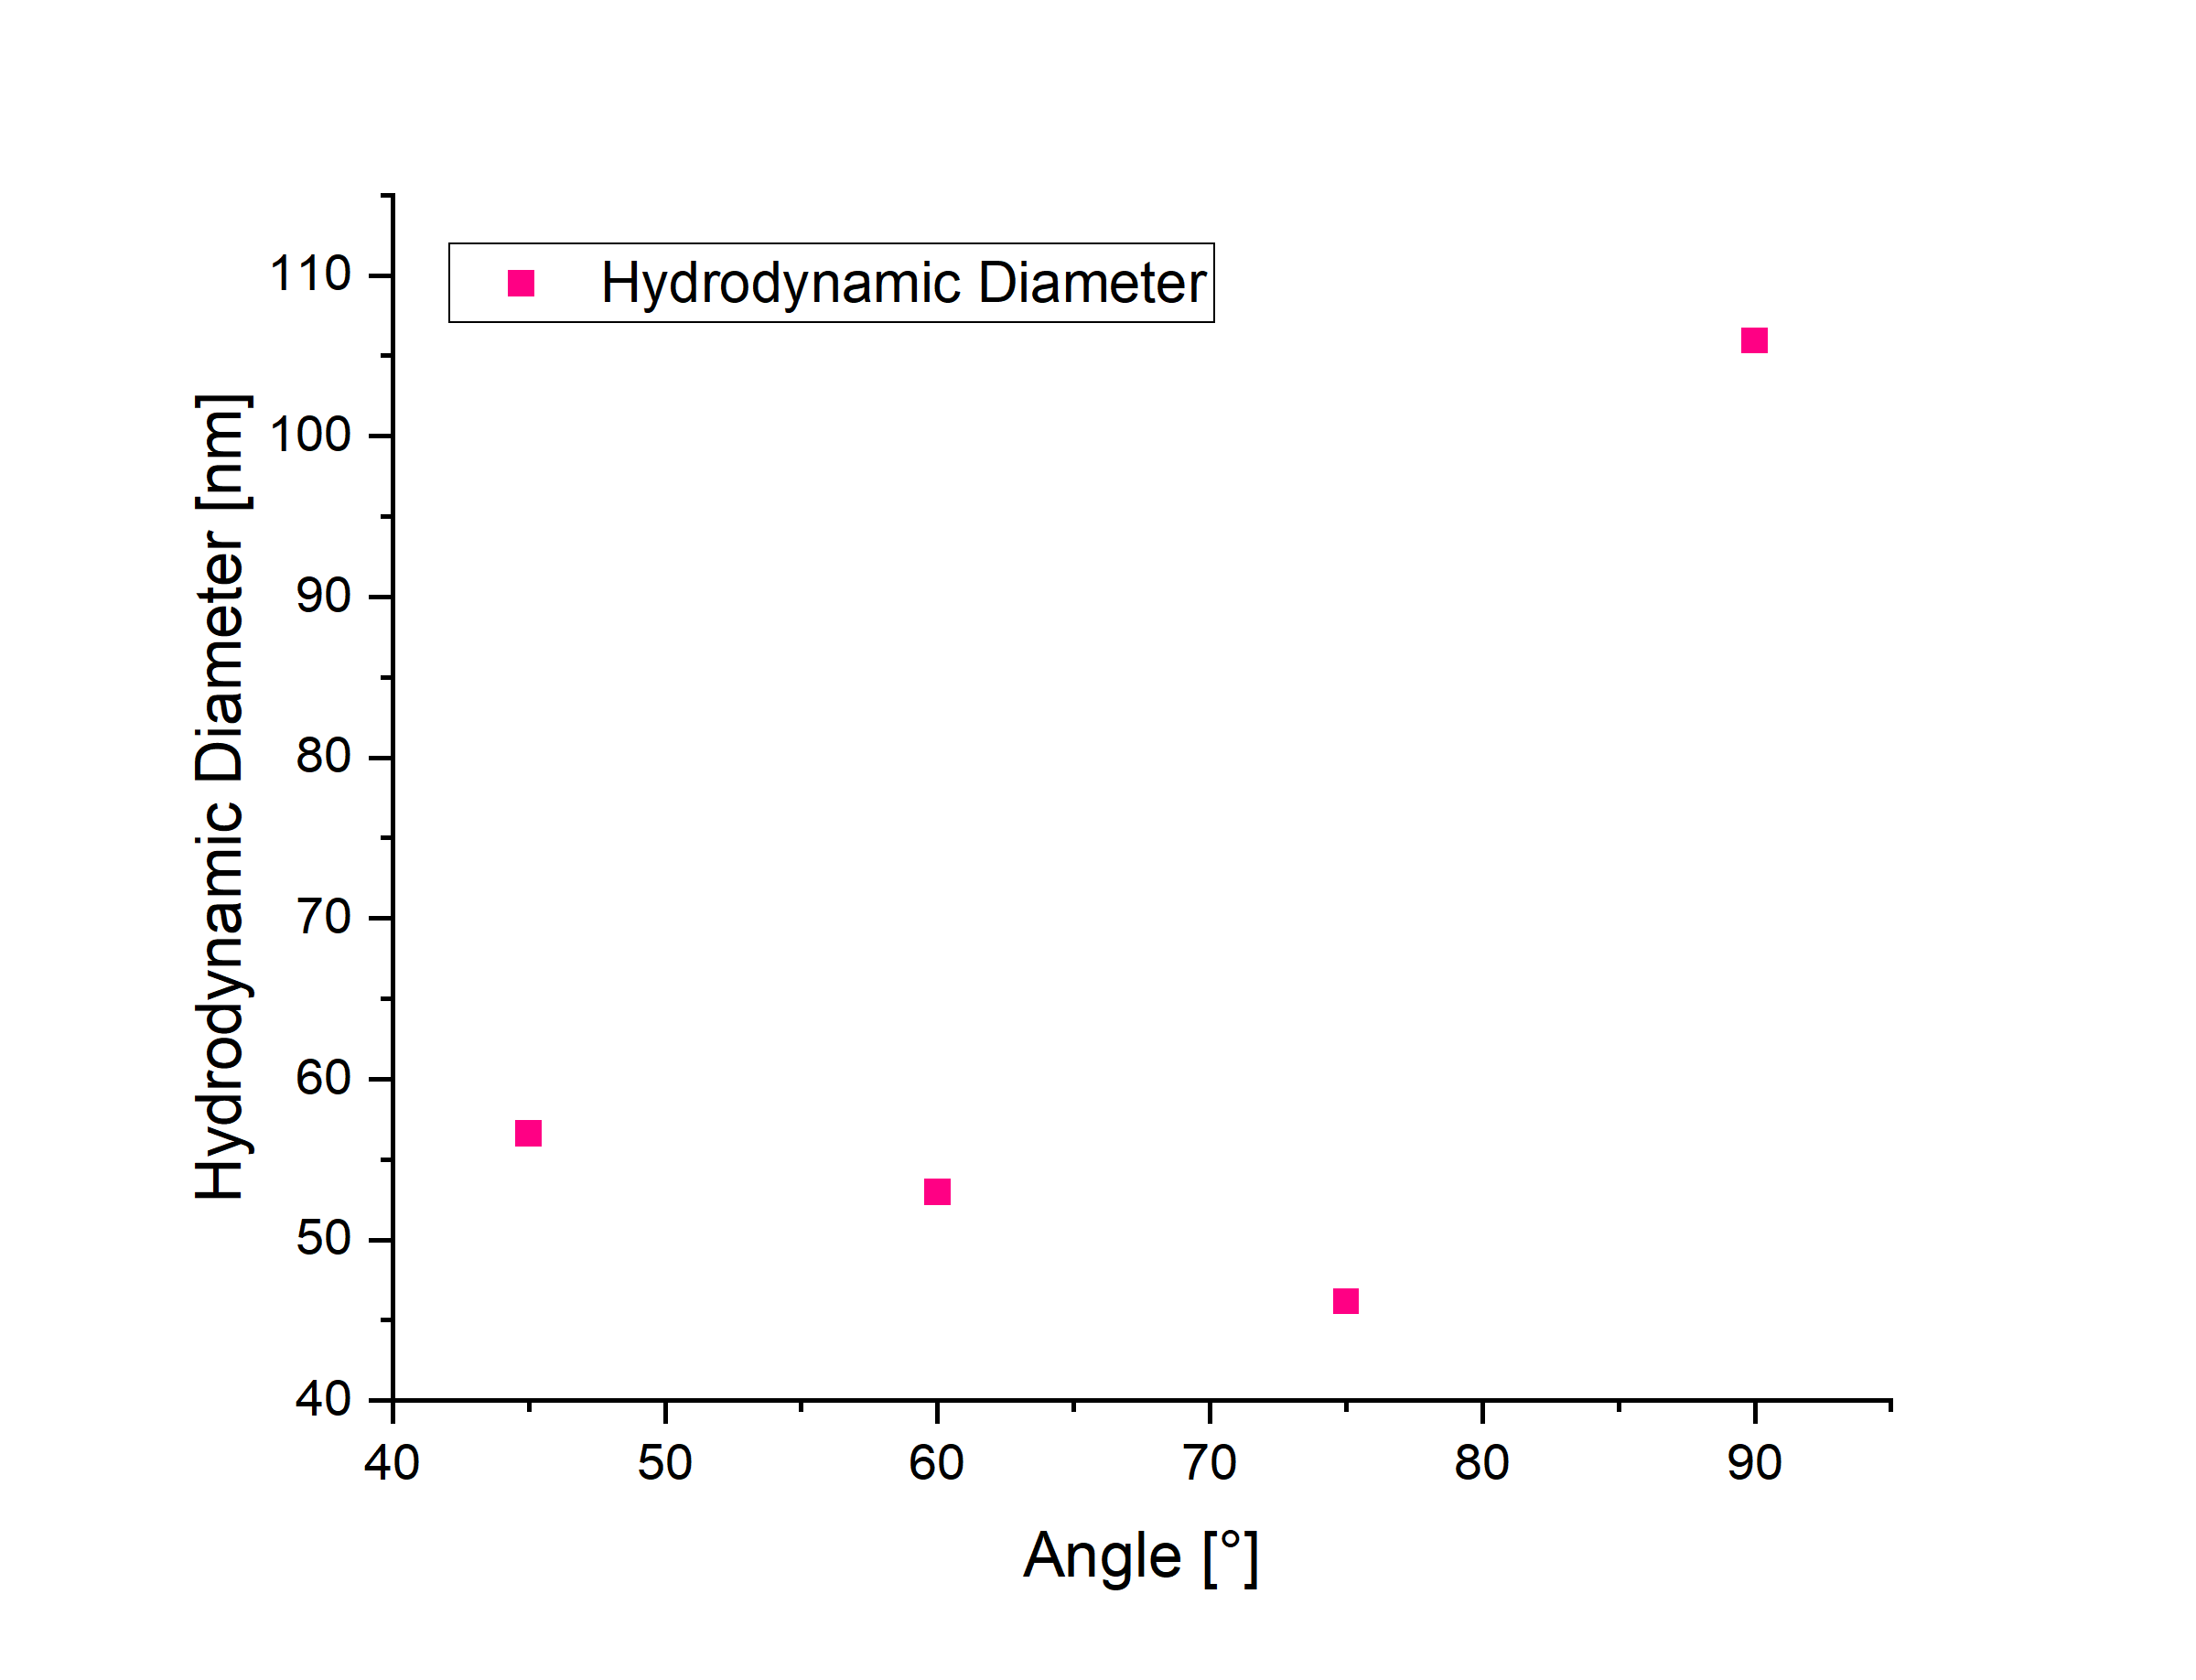
\includegraphics[width=0.8\textwidth]{1_DynamicLightScattering/Graphics/RadiiProbe1.png}
    \caption{Hydrodynamic diameter of sample 1 against scattering angle}
    \label{fig:RadiiProbe1}
\end{figure}
\FloatBarrier

\begin{table}[!ht]
    \centering
    \begin{tabular}{|c|c|}
        \hline
        Scattering Angle (°) & Hydrodynamic Diameter (nm) \\ \hline \hline
        45 & 56.59 \\ \hline
        60 & 52.97 \\ \hline
        75 & 46.17 \\ \hline
        90 & 105.94 \\ \hline
    \end{tabular}
    \caption{Calculated diameters of sample 1 at various scattering angles}
    \label{tab:DiametersSample1}
\end{table}
\FloatBarrier

\subsubsection{Sample 2}

The correlation functions and fits obtained for sample 2 are plotted in fig. \ref{fig:CorrFctProbe2}, and the calculated diameters are presented in fig. \ref{fig:RadiiProbe2} and tab. \ref{tab:DiametersSample2}. The correlation functions are decaying over the same time span, but are well separated by their initial value

As for sample 1, the correlation function is dependent on the scattering angle of the laser, resulting in slight changes of the particle sizes. 

The sample contains particles with a diameter of 460 nm, and while the calculated values are better than with sample 1, we do not reach the correct value.

\begin{figure}[!ht]
    \centering
    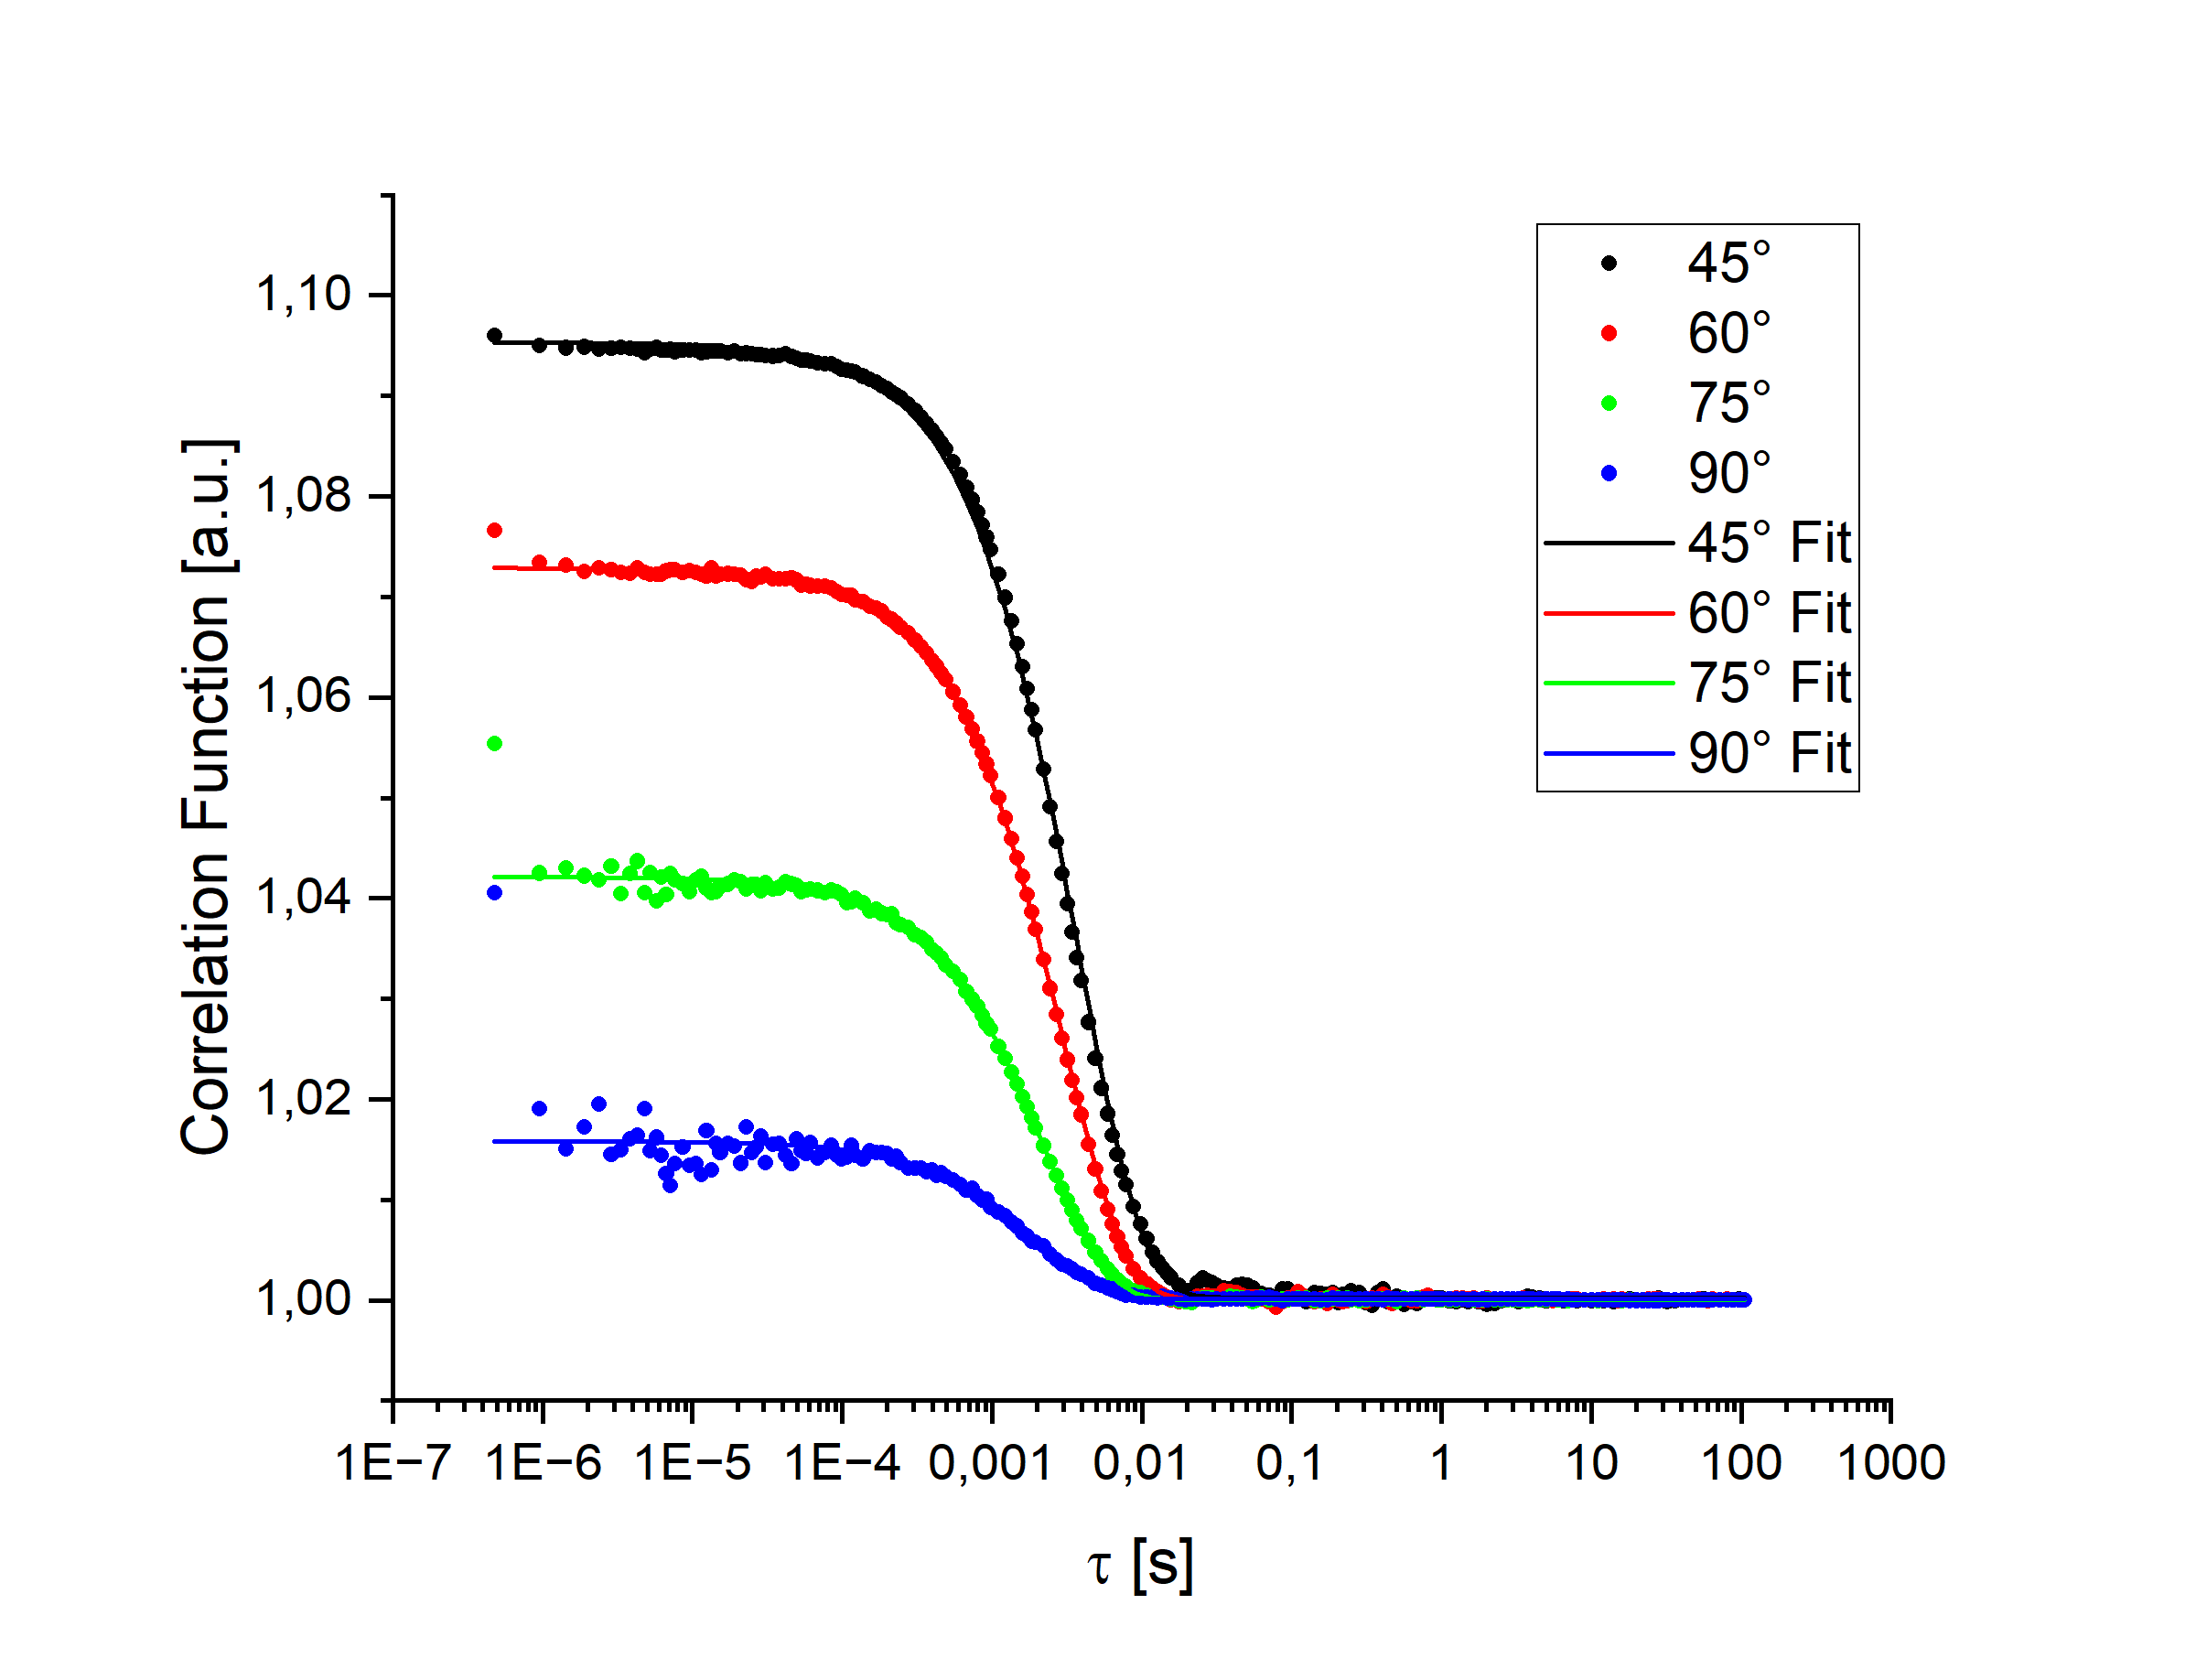
\includegraphics[width=0.8\textwidth]{1_DynamicLightScattering/Graphics/CorrFctProbe2.png}
    \caption{Correlation functions for sample 2 at different scattering angles}
    \label{fig:CorrFctProbe2}
\end{figure}
\FloatBarrier

\begin{figure}[!ht]
    \centering
    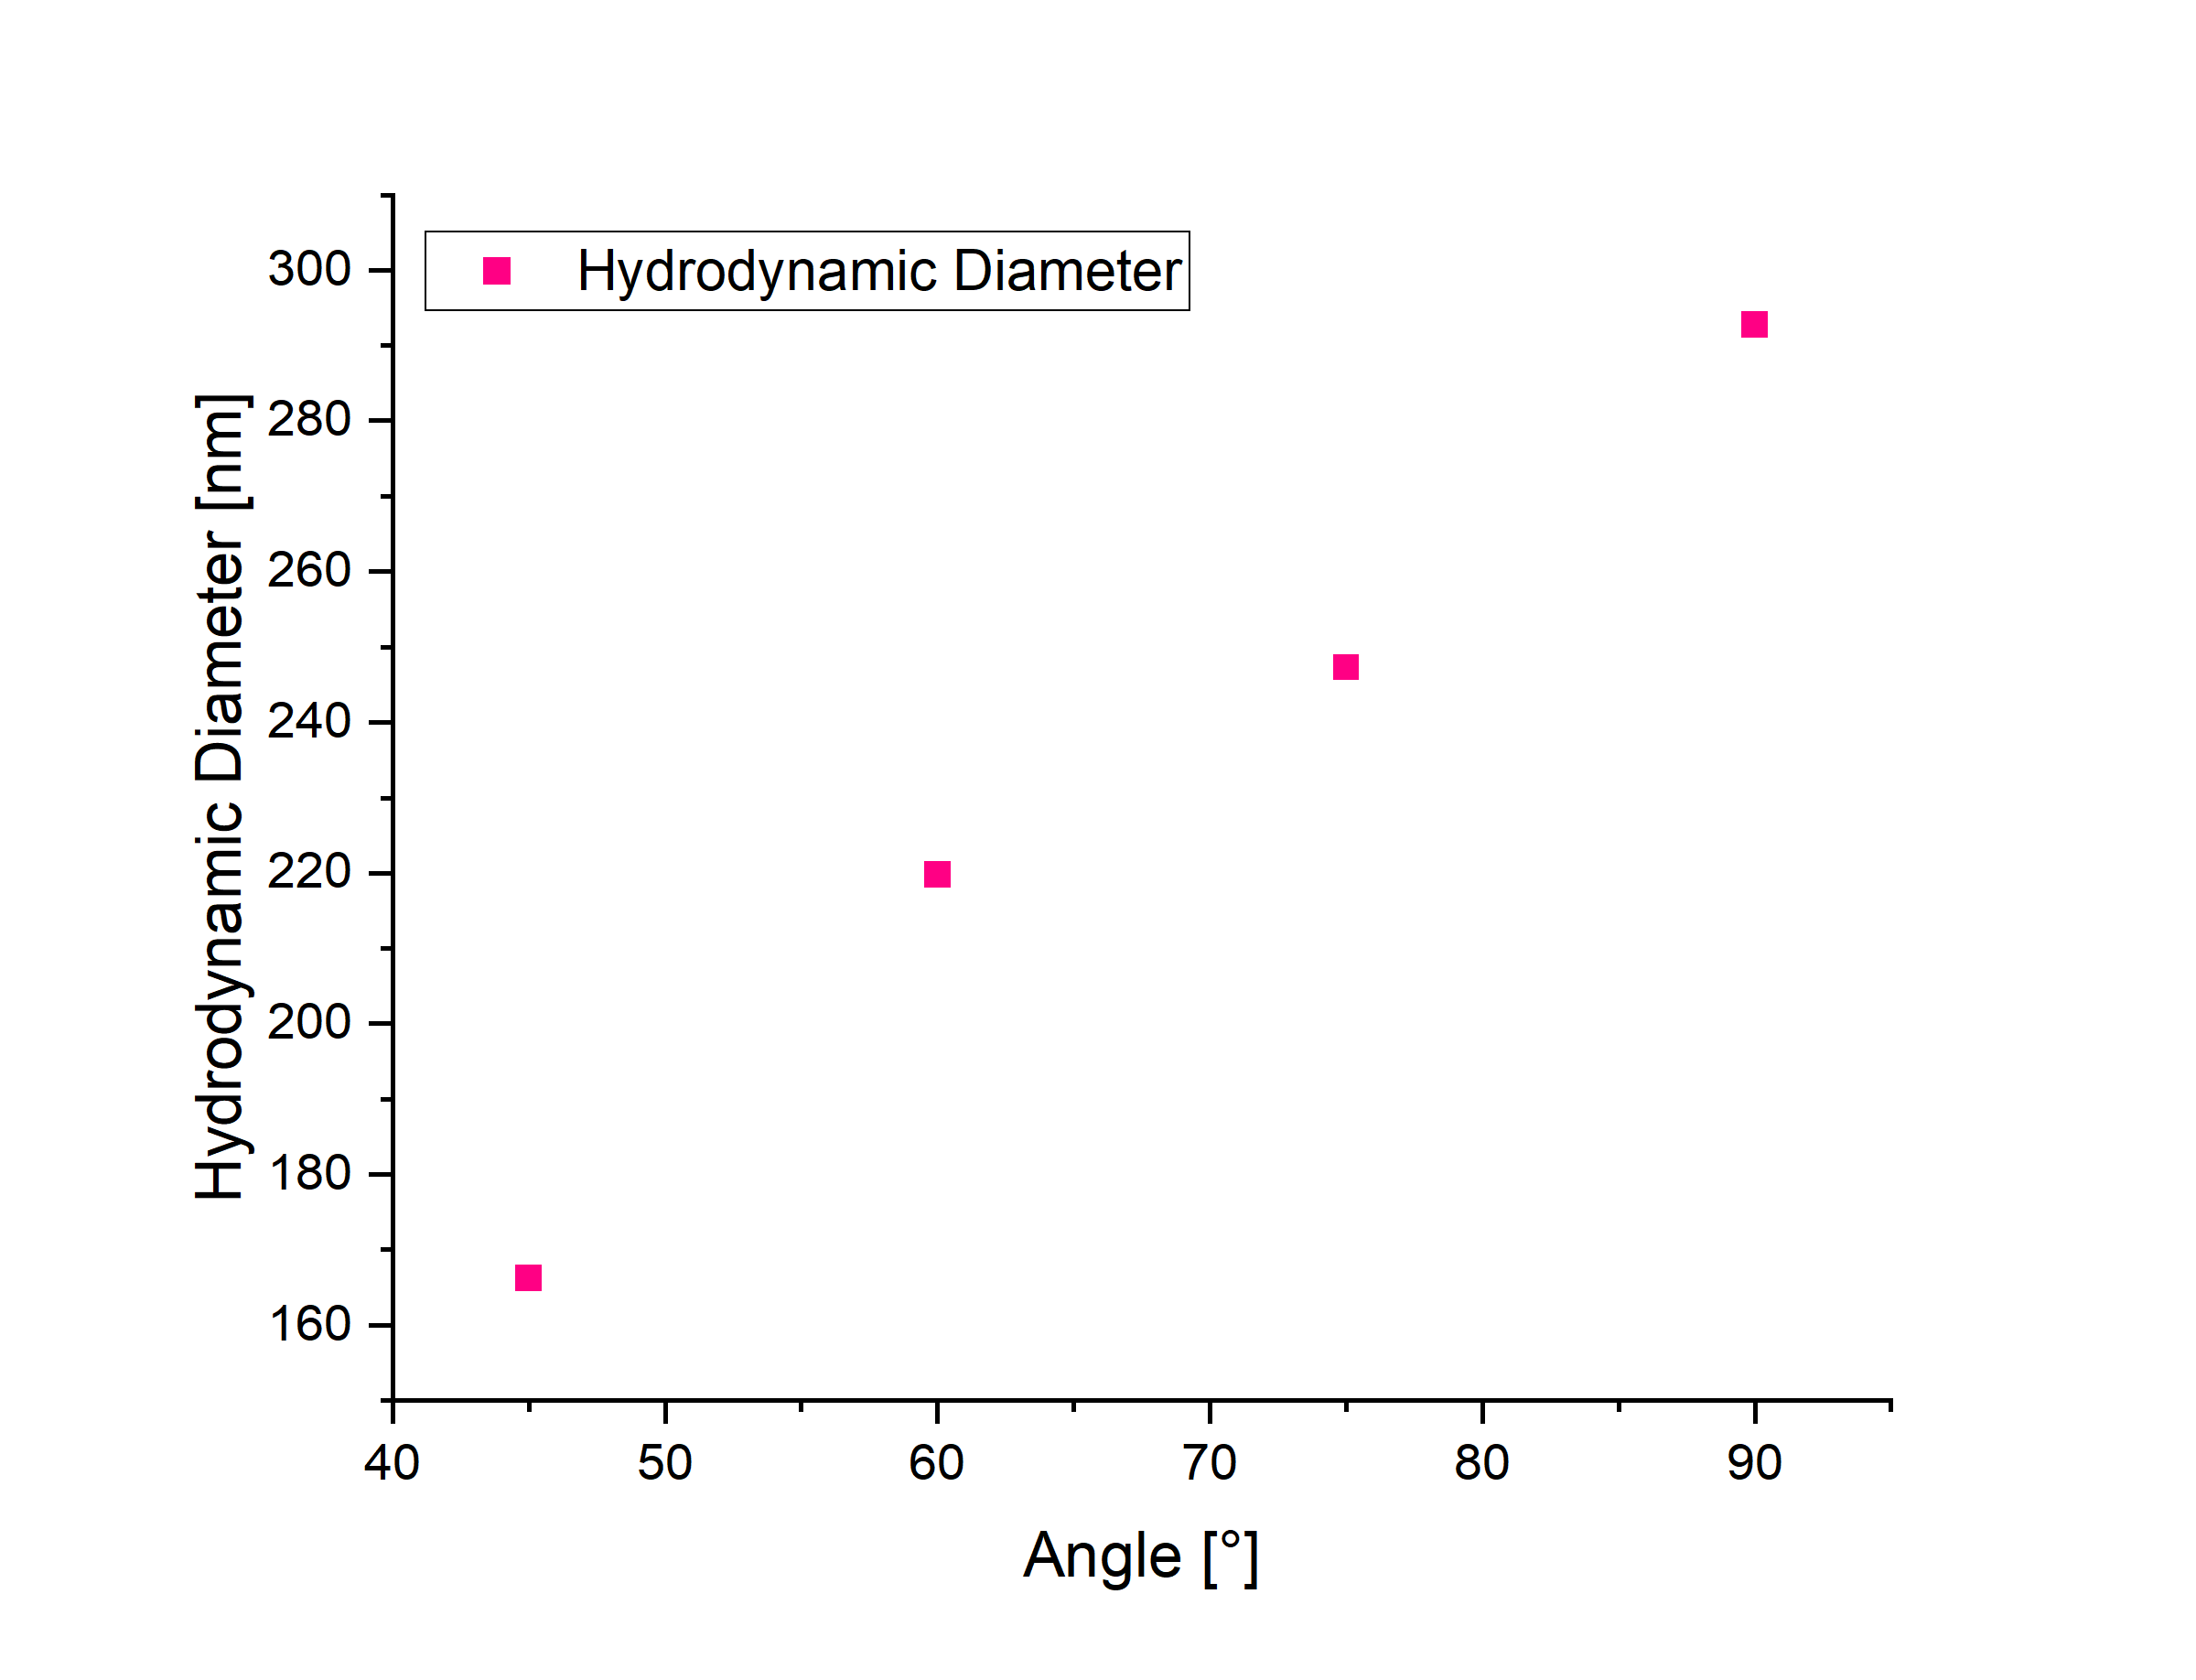
\includegraphics[width=0.8\textwidth]{1_DynamicLightScattering/Graphics/RadiiProbe2.png}
    \caption{Hydrodynamic diameter of sample 2 against scattering angle}
    \label{fig:RadiiProbe2}
\end{figure}
\FloatBarrier

\begin{table}[!ht]
    \centering
    \begin{tabular}{|c|c|}
    \hline
        Scattering Angle (°) & Hydrodynamic Diameter (nm) \\ \hline \hline
        45 & 166.24 \\ \hline
        60 & 219.80 \\ \hline
        75 & 247.30 \\ \hline
        90 & 292.79 \\ \hline
    \end{tabular}
    \caption{Calculated diameters of sample 2 at various scattering angles}
    \label{tab:DiametersSample2}
\end{table}

\subsubsection{Sample 3}
The correlation functions and fits obtained for sample 3 can be found in fig. \ref{fig:CorrFctProbe3}. In contrast to sample 2, the separation of the functions are not as well separated.
Nonetheless, we can calculate the diameter of the particles, which are presented in fig. \ref{fig:RadiiProbe3} and tab. \ref{tab:DiametersSample3}. The sample contains particles with a diameter of 10 nm, and our values are getting close, but indicate a bigger particle size.
An angular dependency of the correlation function and the computed particle diameter is yet again visible.

\begin{figure}[!ht]
    \centering
    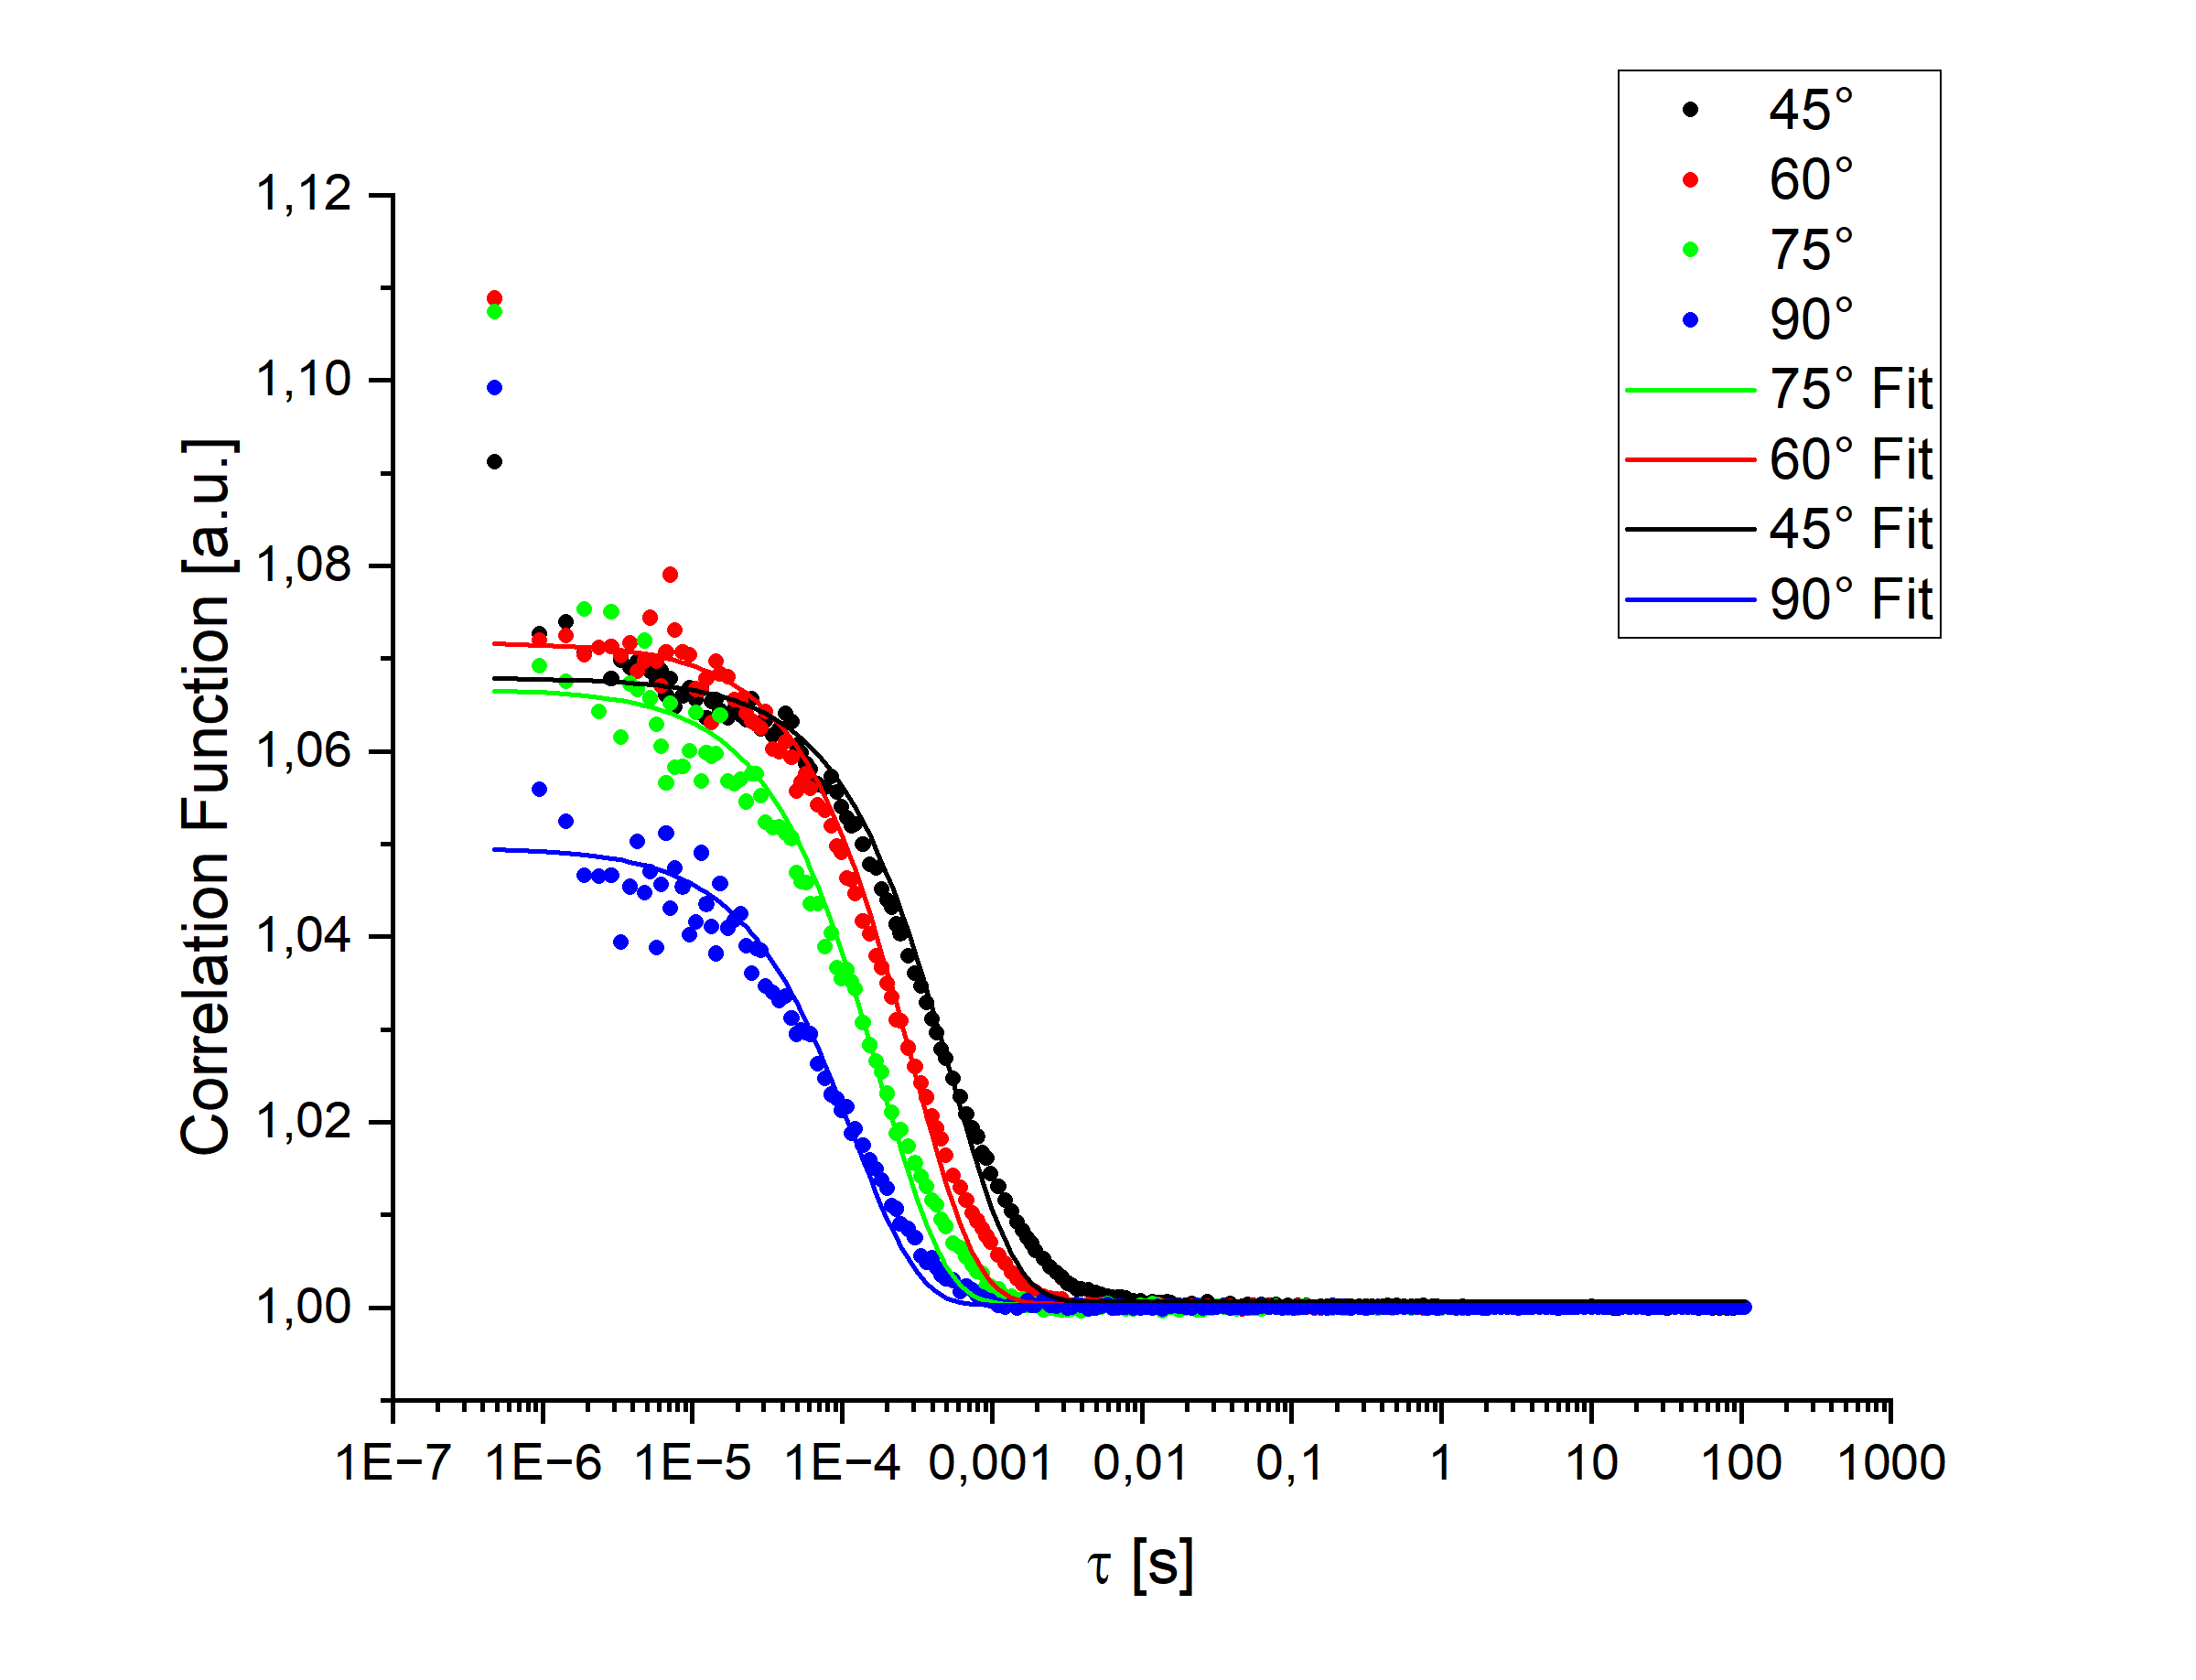
\includegraphics[width=0.8\textwidth]{1_DynamicLightScattering/Graphics/CorrFctProbe3.png}
    \caption{Correlation functions for sample 3 at different scattering angles}
    \label{fig:CorrFctProbe3}
\end{figure}
\FloatBarrier

\begin{figure}[!ht]
    \centering
    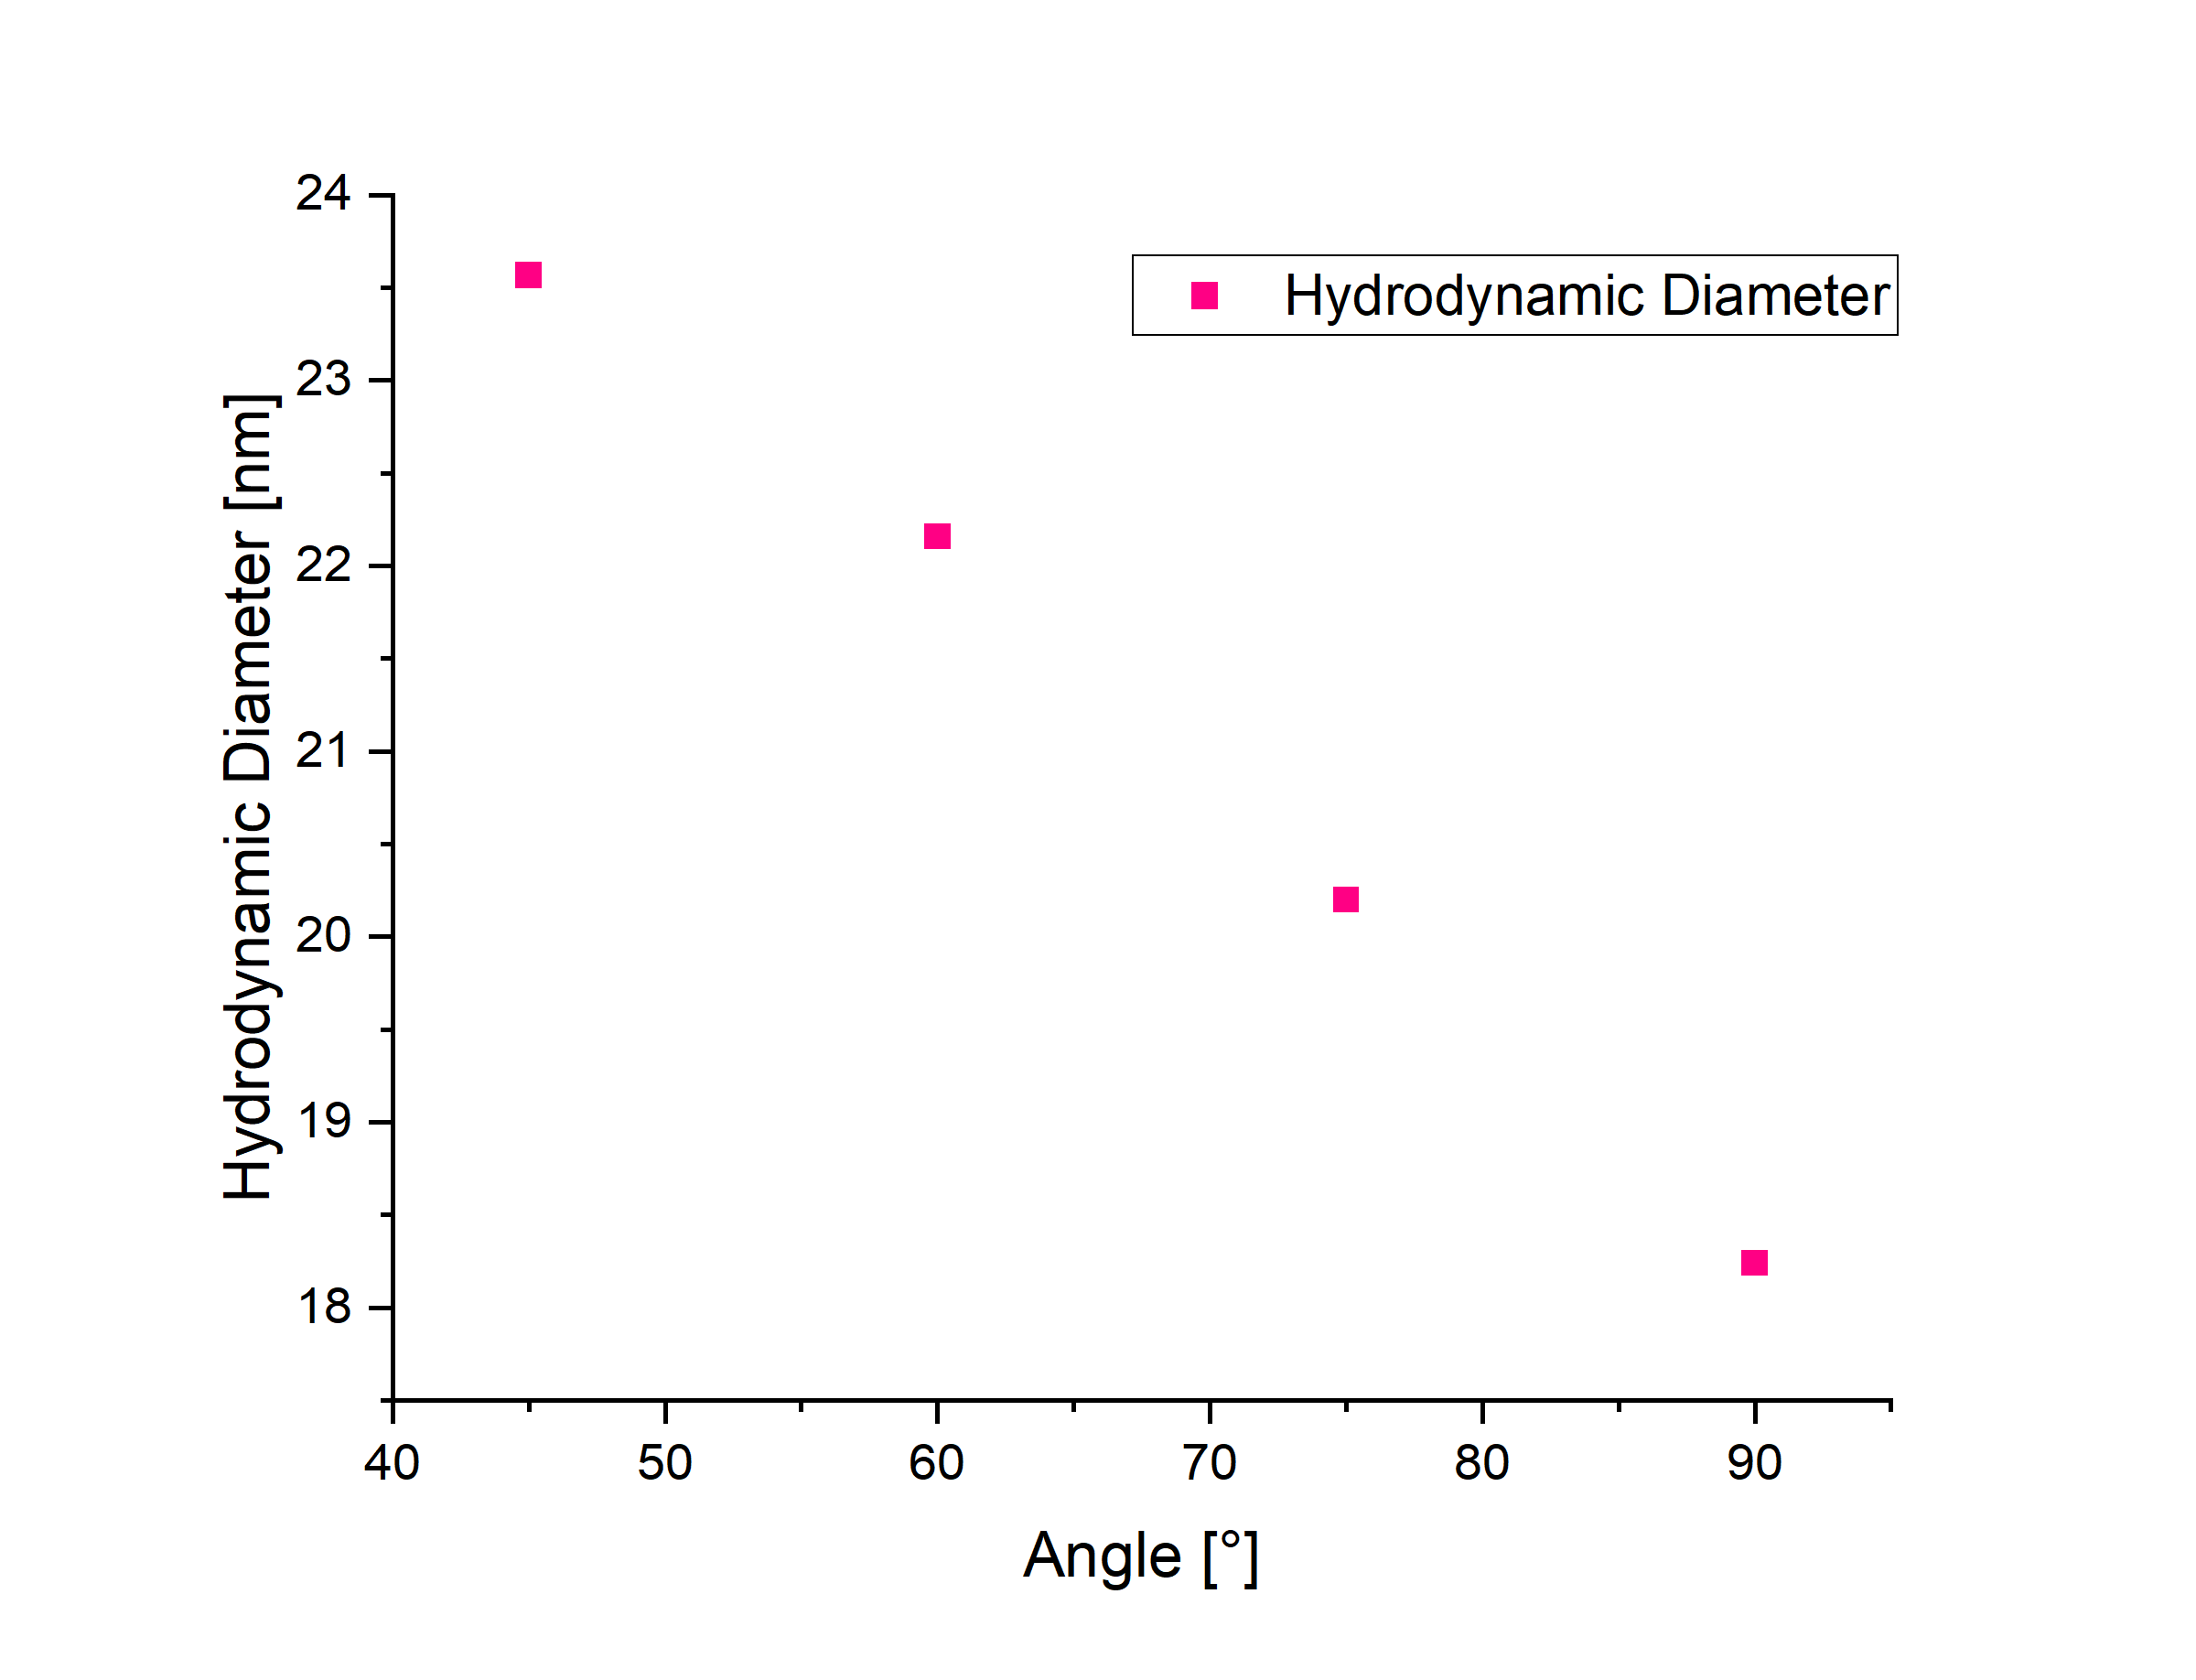
\includegraphics[width=0.8\textwidth]{1_DynamicLightScattering/Graphics/RadiiProbe3.png}
    \caption{Hydrodynamic diameter of sample 3 against scattering angle}
    \label{fig:RadiiProbe3}
\end{figure}
\FloatBarrier

\begin{table}[!ht]
    \centering
    \begin{tabular}{|c|c|}
    \hline
        Scattering Angle (°) & Hydrodynamic Diameter (nm) \\ \hline \hline
        45 & 23.57 \\ \hline
        60 & 22.16 \\ \hline
        75 & 20.20 \\ \hline
        90 & 18.24 \\ \hline
    \end{tabular}
    \caption{Calculated diameters of sample 3 at various scattering angles}
    \label{tab:DiametersSample3}
\end{table}
\FloatBarrier

\subsection{Concentration dependency}

In this section we try to study the influence of the concentration of particles in solution on the correlation function. We fix the scattering angle at 90°. The samples 5 and 6 are diluted from sample 1. As can be seen in fig. \ref{fig:Probe1+5+6}, the correlation function obtained from sample 5 \& 6 is near unusable. The data even seems to exhibit a sinusoidal tendency. 

Calculating the diameter of the particles also yields nonsensical values, which can be found in tab. \ref{tab:DiametersSample1+5+6}.

Maybe the critical concentration has already been reached, where the analysis isn't possible anymore. It is hard to draw other conclusions from the data.

What we would expect is that the correlation function changes with the concentration. If the particle concentration is very high in the solution, the particles interact much more strongly with each other. As the concentration diminishes, we would observe less and less of those interactions. This change would be lead to a different value of the diffusion coefficient.

\begin{figure}[!ht]
    \centering
    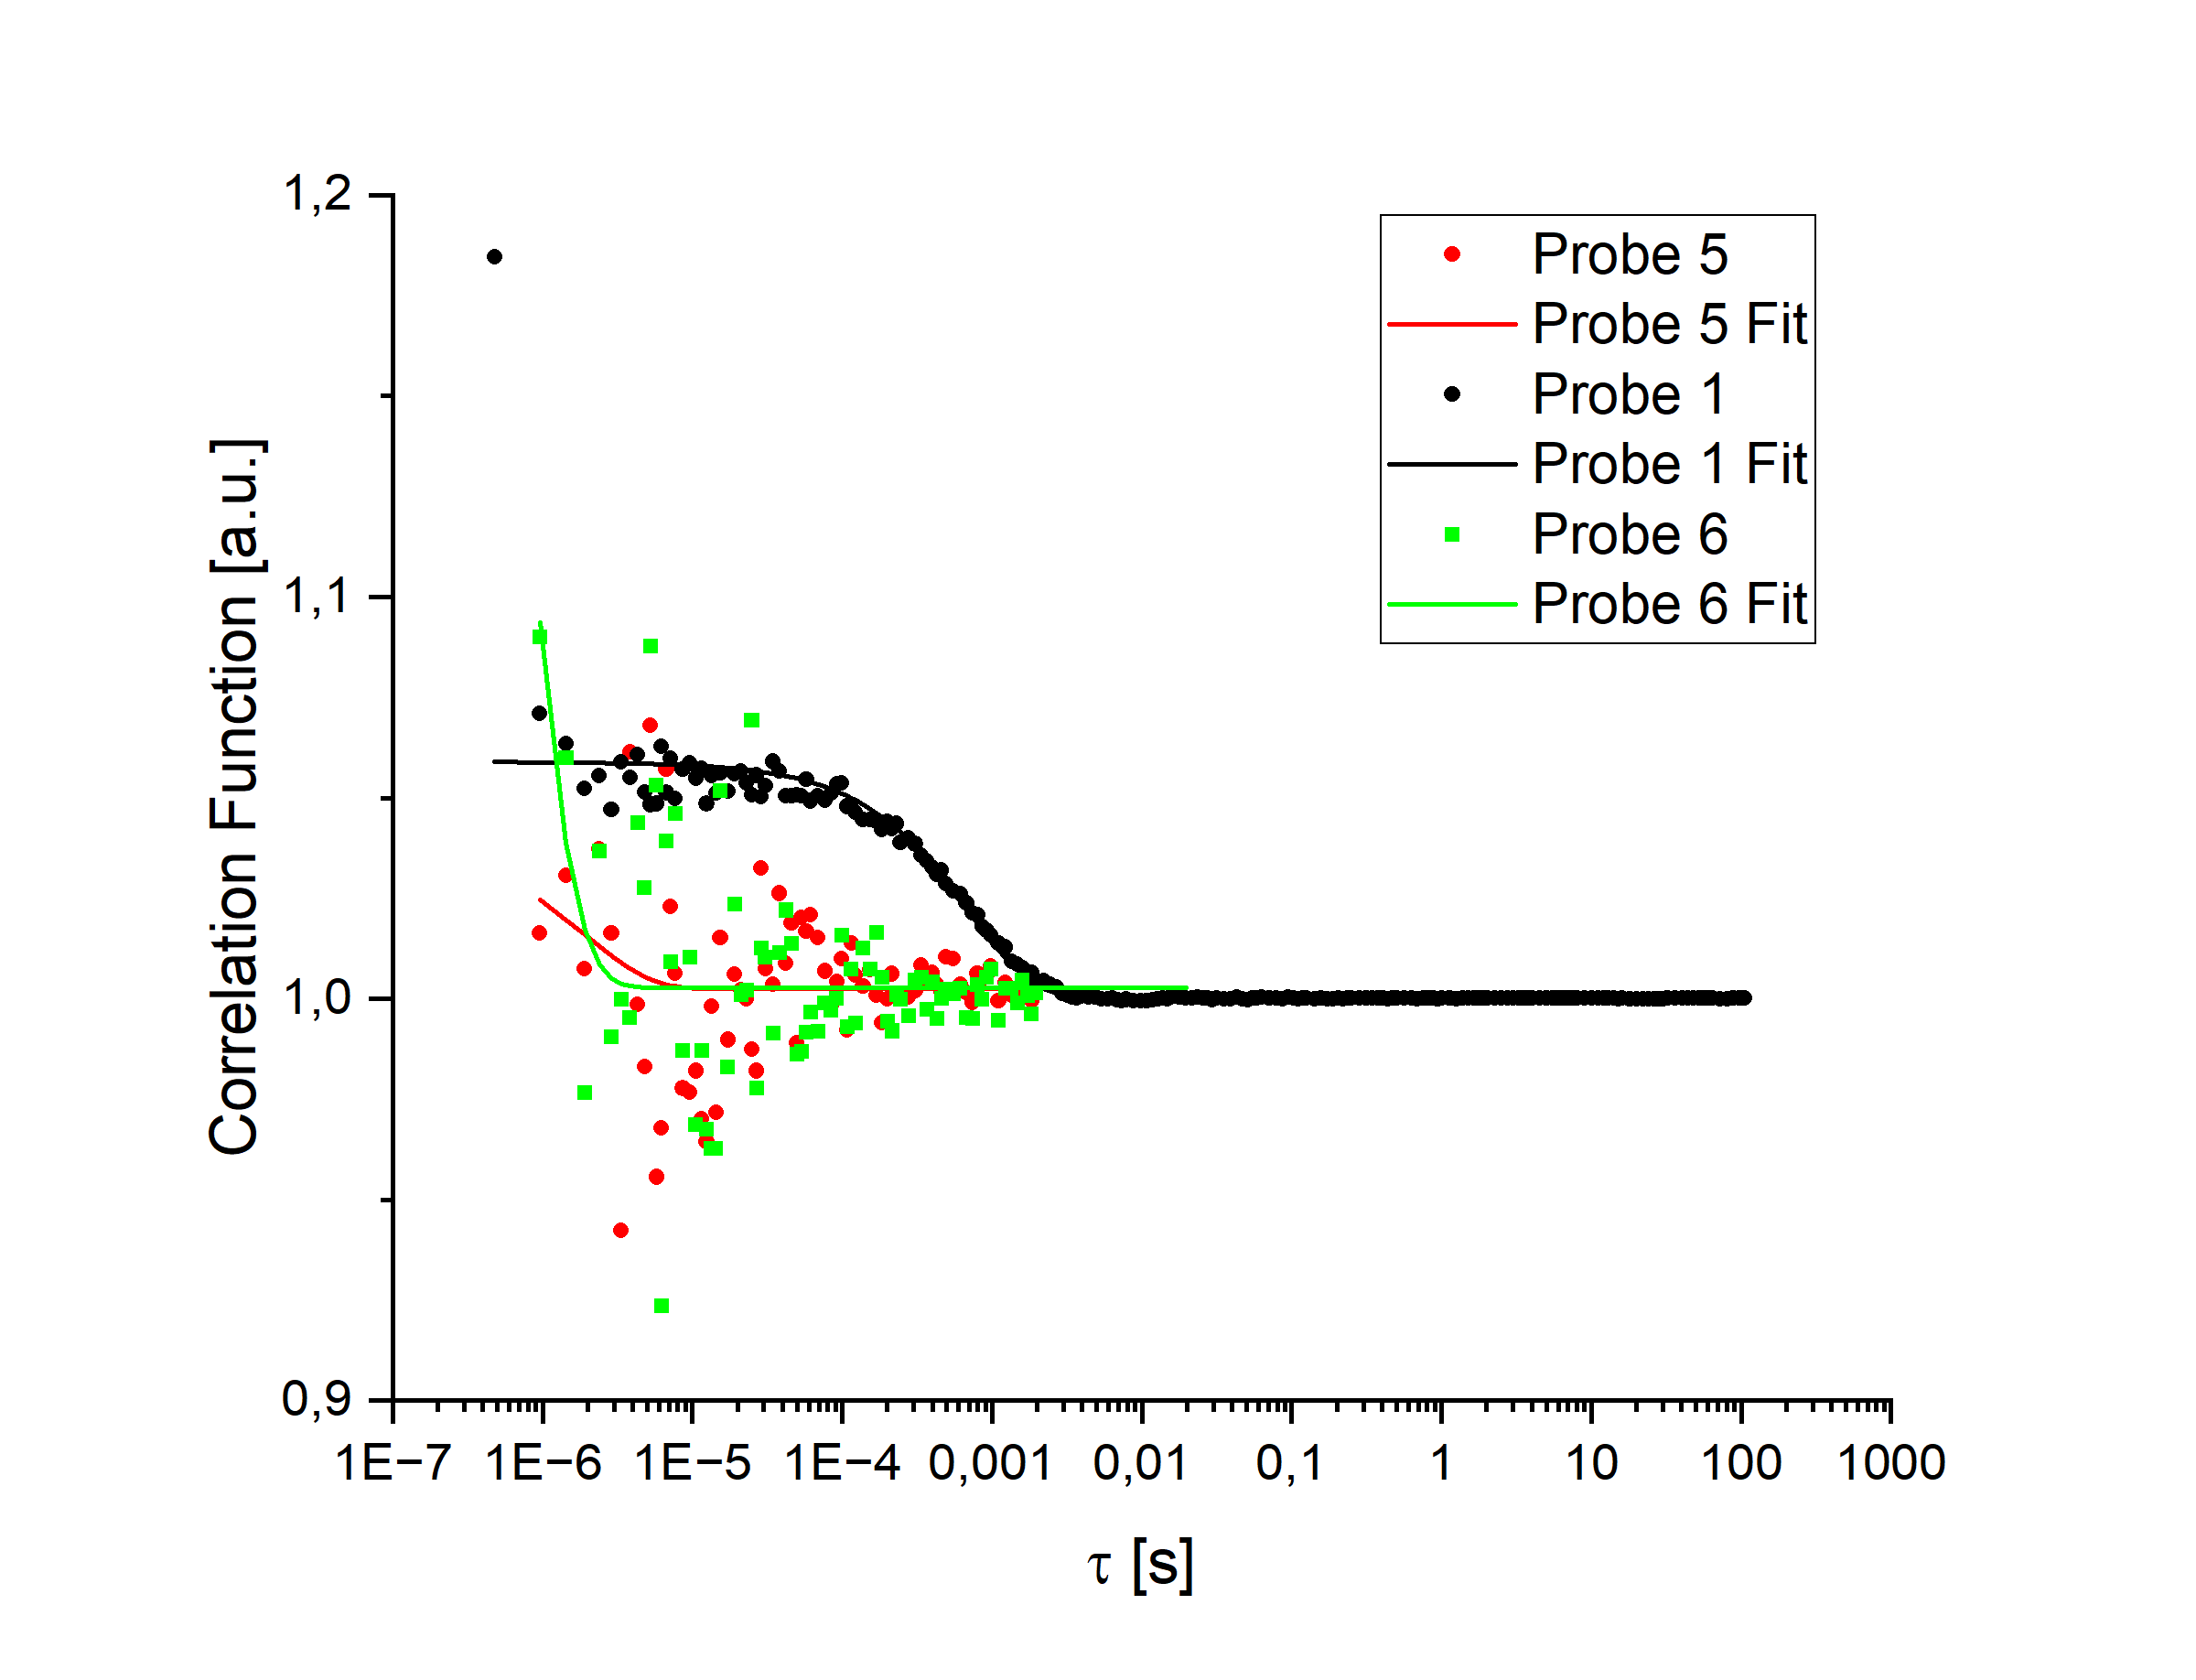
\includegraphics[width=0.8\textwidth]{1_DynamicLightScattering/Graphics/CorrFctProbe1+5+6.png}
    \caption{Correlation functions for sample 1, 5 and 6 at 90° scattering angle}
    \label{fig:Probe1+5+6}
\end{figure}
\FloatBarrier

\begin{table}[!ht]
    \centering
    \begin{tabular}{|c|c|}
    \hline
        sample & Hydrodynamic Diameter (nm) \\ \hline \hline
        1 & 105.94 \\ \hline
        5 & 0.30 \\ \hline
        6 & 0.08 \\ \hline
    \end{tabular}
    \caption{Calculated diameters of sample 1, 5 and 6 at a scattering angle of 90°}
    \label{tab:DiametersSample1+5+6}
\end{table}

\subsection{Poly-disperse samples}

In this section we compare a solution containing particles of two different sizes in equal proportions, to the solutions containing particles of only one size. sample 7 contains a mixture of the beads from sample 1 and sample 2. As seen in fig. \ref{fig:Probe1+2+7}, the obtained correlation function is not simply the sum of the two correlation functions. The calculated diameters using the fit function for two particle sizes (eq. \ref{eq:DoubleParticleFit}) can be found in tab. \ref{tab:DiametersSample1+2+7}. Interestingly, the sample 7 behaves as if it were containing one very big particle, and one very small one; the difference in order of magnitude is about 10000. The big particle's diameter is approximately the average of the diameters of the two particle sizes. The sample seems to behave as a mono-disperse sample, rather than a poly-disperse one. It is also not exactly the phenomenon where the scattered light from the bigger particle eclipses the scattered light from the smaller particle, as we would expect to get the correlation function of the bigger particle and not of the average size particle.

\begin{figure}[!ht]
    \centering
    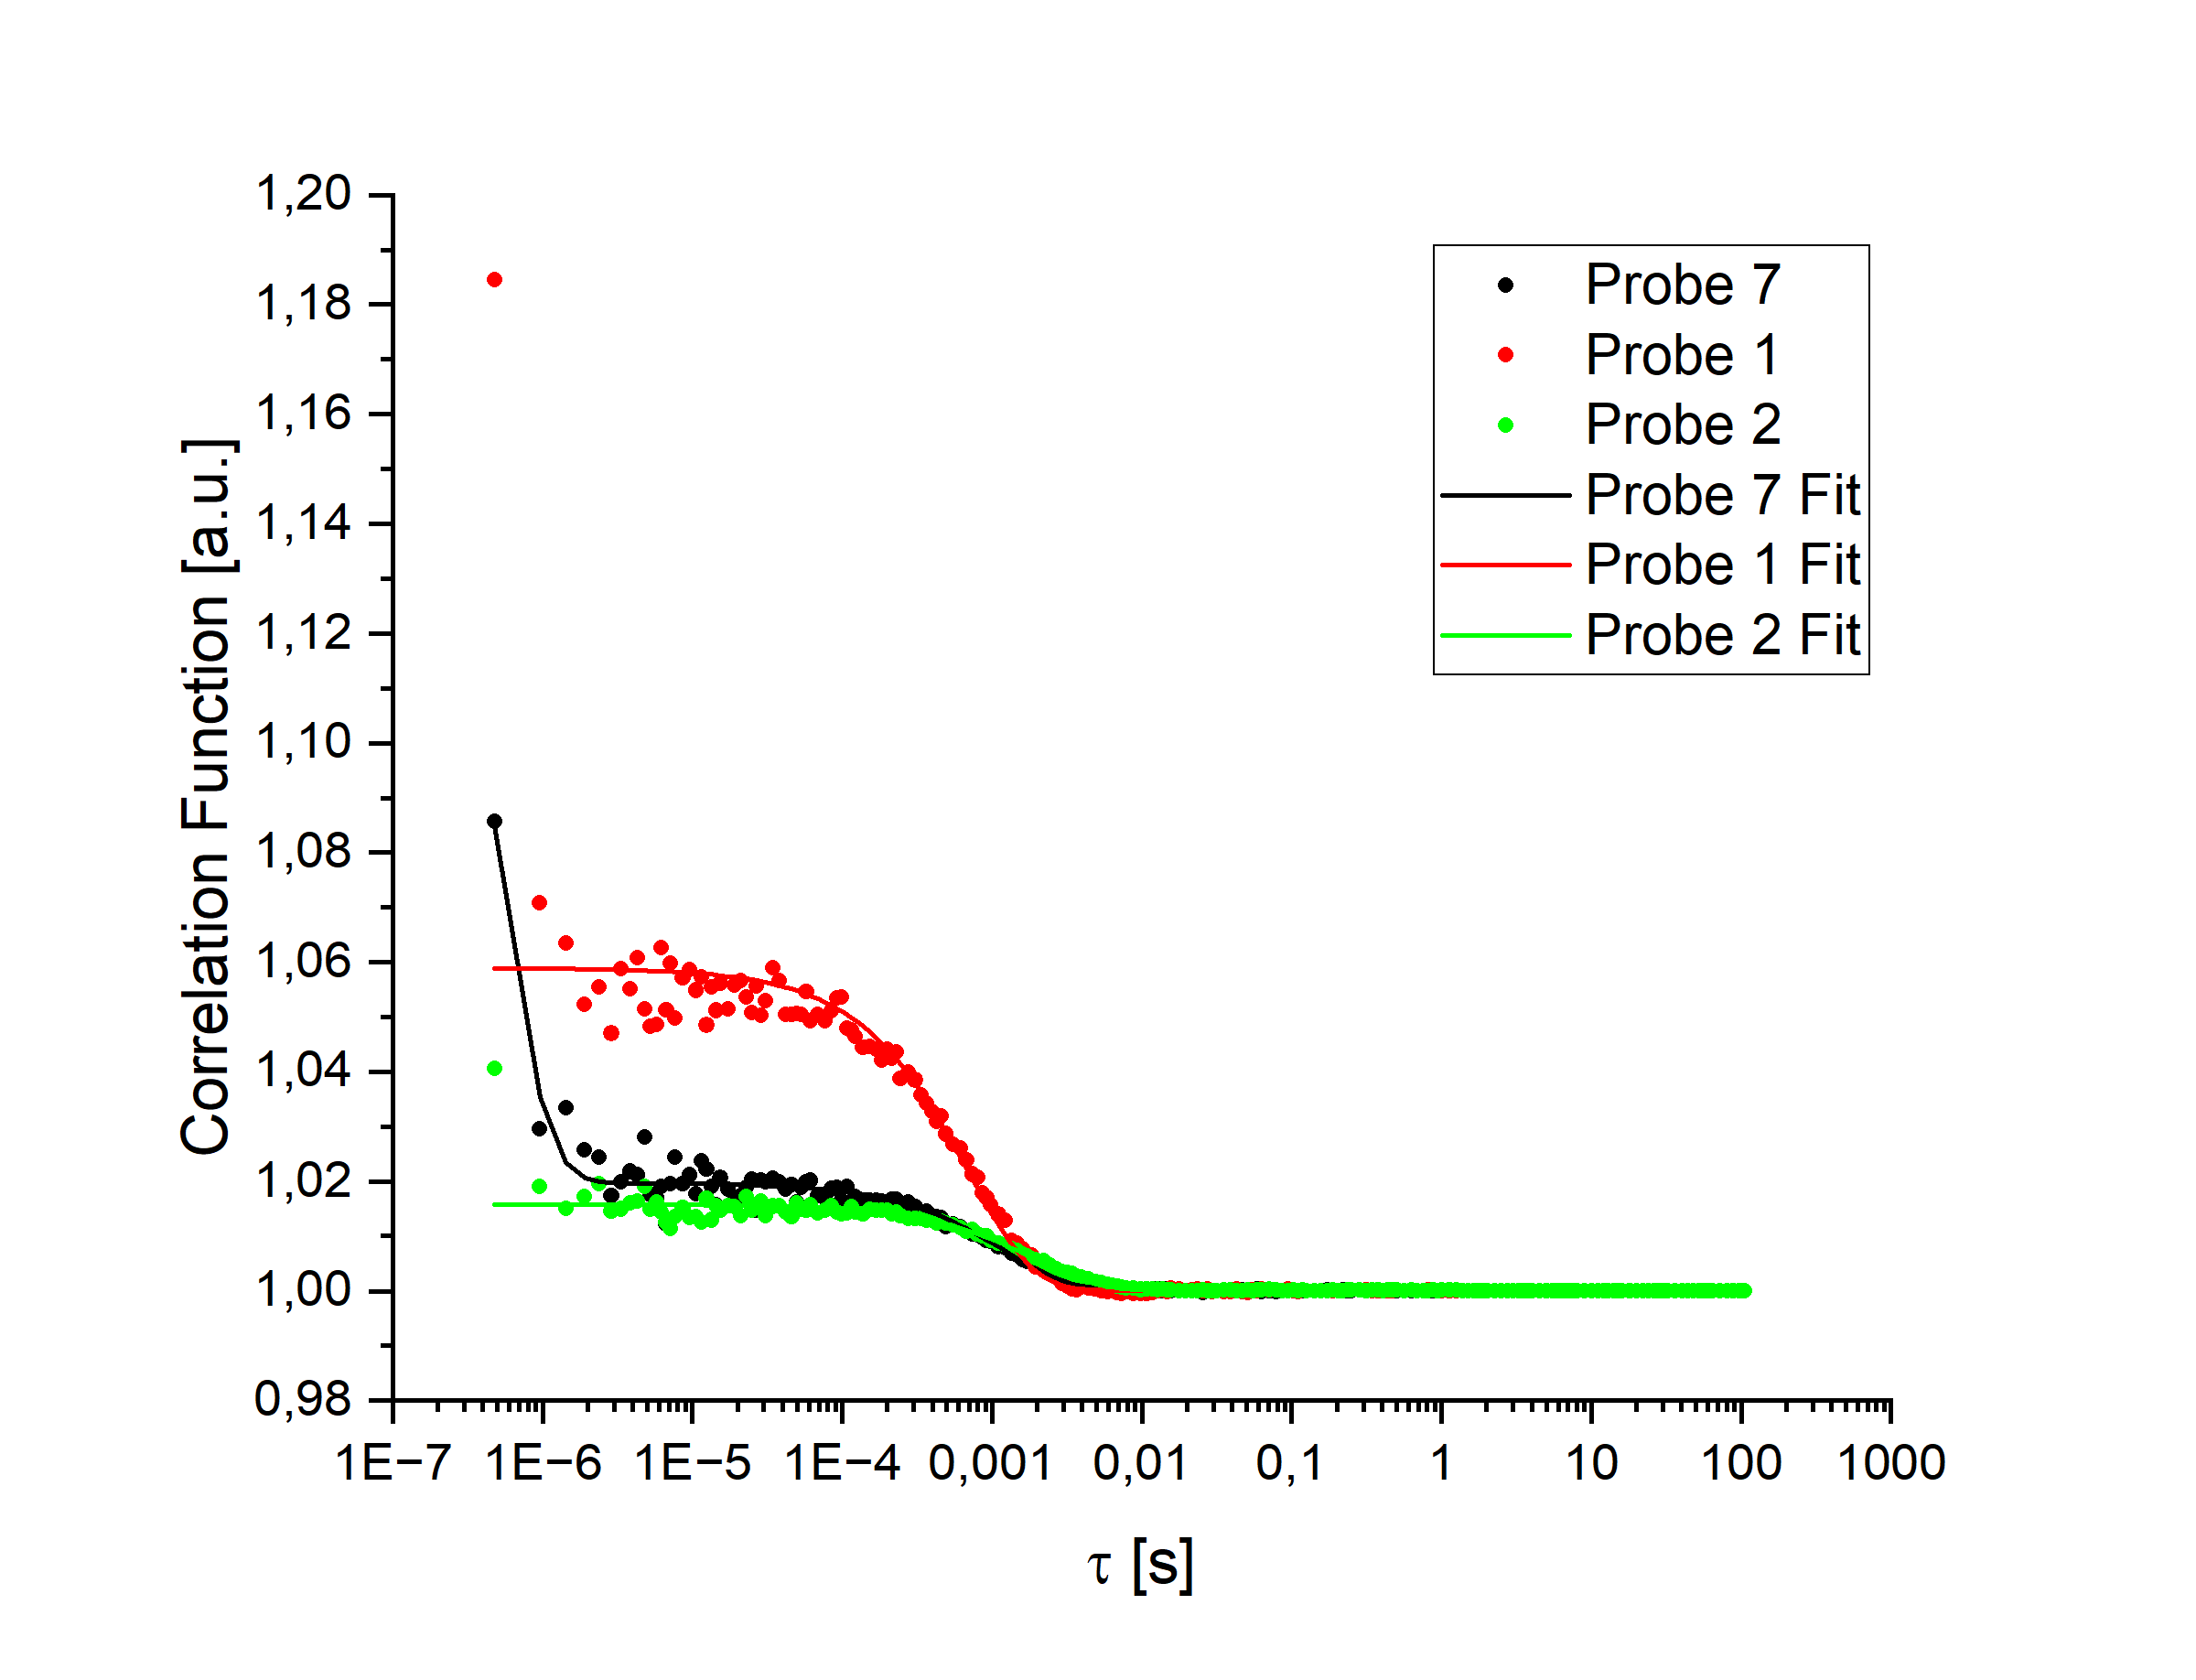
\includegraphics[width=0.8\textwidth]{1_DynamicLightScattering/Graphics/CorrFctProbe1+2+7.png}
    \caption{Correlation functions for sample 1, 2 and 7 at 90° scattering angle}
    \label{fig:Probe1+2+7}
\end{figure}
\FloatBarrier

\begin{table}[!ht]
    \centering
    \begin{tabular}{|c|c|c|}
    \hline
        sample Number & Hydrodynamic Diameter 1 (nm) & Hydrodynamic Diameter 2 (nm) \\ \hline \hline
        1 & 105.94 & ~ \\ \hline
        2 & ~ & 292.79 \\ \hline
        7 & 0,05134 & 186.83 \\ \hline
    \end{tabular}
    \caption{Calculated diameters of sample 1, 2 and 7 at a scattering angle of 90°}
    \label{tab:DiametersSample1+2+7}
\end{table}

\section{Conclusion}

In this experiment we have recorded and analyzed the dynamic light scattering on solutions containing latex and ludox particles. We have shown that the obtained correlation function depends on the scattering angle and on the concentration of the particles in the sample. We have further calculated the particle sizes and while approaching them, our results were off by a significant amount from the actual values.

It is difficult to do a qualitative analysis of the concentration dependency, as there were no indications of the concentrations of the beads in the mother solutions. When diluting the solutions we may have extracted some sample with little to no beads in them. The beads are supposedly in suspension, but may have accumulated in a certain spot after waiting for too long.  Also some of the solutions had a high viscosity, and we did not manage to get the exact volume into the sample tube. This could have been remedied by heating the solution, which would have lowered its viscosity.

A few possible improvements would be to include ways to verify the concentrations of beads in the solutions, starting with correct labels on their containers. Optical microscopes would not have the resolution power to be able to quickly look at a sample from the solution to verify the presence of the beads, and another method would be necessary.

\nocite{LabGuideDLS}
\nocite{introDLS}
\nocite{DLStraining}
\nocite{DLSPracticalGuide}

\printbibliography


\end{document}